\documentclass[lettersize,journal]{IEEEtran}

\usepackage{amsmath,amsfonts}
\usepackage{array}
\usepackage{booktabs}
\usepackage{cite}
\usepackage{graphicx}
\usepackage{microtype}
\usepackage{multirow}
\usepackage{stfloats}
\usepackage{placeins}
\usepackage{xspace}
\usepackage{xurl}
\usepackage[hidelinks]{hyperref}
\usepackage{etoolbox}
\graphicspath{{figures/}}

\newcommand{\model}{MCGI-YOLO\xspace}
\newcolumntype{L}[1]{>{\raggedright\arraybackslash}p{#1}}

\setlength{\textfloatsep}{12pt plus 2pt minus 2pt}
\setlength{\dbltextfloatsep}{12pt plus 2pt minus 2pt}
\setlength{\floatsep}{10pt plus 2pt minus 2pt}
\setlength{\dblfloatsep}{10pt plus 2pt minus 2pt}

\begin{document}
\raggedbottom

\title{A Defect Detection and Closed-Loop Control System with MCGI-YOLO for Circular Knitting Machines}

\author{Kangzhao Tan, Jiarui Zhang, Junjie Yu, Heng Wu, Jing Lin\textsuperscript{*}, Diyu Li\textsuperscript{*}, and Chunhua He\textsuperscript{*}%
\thanks{Manuscript received xxxx xx, xxxx; revised xxxx xx, xxxx; accepted xxxx xx, xxxx. This work was supported in part by the National Natural Science Foundation of China under Grant U22A2012. \textit{(\textsuperscript{*}Corresponding authors: Jing Lin, Diyu Li, and Chunhua He.)}}%
\thanks{\begingroup\urlstyle{same}Kangzhao Tan, Jiarui Zhang, Junjie Yu, and Chunhua He are with the School of Computer Science, Guangdong University of Technology, Guangzhou 510006, China (e-mail: \protect\url{tankangzhao@mails.gdut.edu.cn}; \protect\url{zhangjiarui1@mails.gdut.edu.cn}; \protect\url{yujunjie2@mails.gdut.edu.cn}; \protect\url{hechunhua@pku.edu.cn}). Heng Wu is with the School of Automation, Guangdong University of Technology, Guangzhou 510006, China (e-mail: \protect\url{heng.wu@gdut.edu.cn}). Jing Lin is with the Classroom Management Center, Guangdong University of Technology, Guangzhou 510006, China (e-mail: \protect\url{lj@gdut.edu.cn}). Diyu Li is with Guangzhou Vinsome Automation Technology Co., Ltd., Guangzhou, China (e-mail: \protect\url{lidiyu@vinsome.cn}).\endgroup}%
}

\maketitle

\begin{abstract}
Defect detection is critical for circular knitting production, where persistent needle or yarn abnormalities lead to repeated fabric defects, resulting in severe material waste and economic losses. Existing methods are rarely tailored to circular knitting machines and tend to be cost-prohibitive, limiting large-scale industrial deployment. To address this issue, we present a low-cost, dedicated defect detection and closed-loop control system for circular knitting machines, which triggers image acquisition from machine rotation, halts the machine upon defect detection to interrupt defect propagation, and alerts the operator for corrective intervention, forming a complete production–detection–control loop. To further improve detection accuracy for diverse fabric defect morphologies and scales, we propose a lightweight detector termed \model. To strengthen boundary evidence against repetitive fabric texture, selective gradient residual enhancement (SGRE) learns to select and mix fixed gradient responses after each bottleneck in the P3 and P4 backbone stages. To reconstruct fine spatial responses with limited computation, subpixel-adaptive residual upsampling (SARU) adds a low-resolution filtered correction with content-dependent weights for the four upsampled positions. On a real-world dataset collected from a circular-knitting production line, \model achieves 97.4\% mAP50 and 65.5\% mAP50--95, improving on the YOLOv8n baseline by 6.9 and 7.1 percentage points, respectively. The model achieves a pure-inference throughput of 491 FPS on an RTX 3090 at FP32 precision and batch size 1. The proposed system provides a cost-effective solution for real-time defect detection in circular-knitting production.
\end{abstract}

\begin{IEEEkeywords}
Circular knitting machine, edge computing, fabric defect detection, selective gradient residual enhancement (SGRE), subpixel-adaptive residual upsampling (SARU), YOLO.
\end{IEEEkeywords}

\markboth{IEEE INTERNET OF THINGS JOURNAL}{}

\section{Introduction}
\IEEEPARstart{C}{ircular} knitting machines are key production equipment for high-volume weft-knit fabric, which is widely used in everyday clothing such as T-shirts and sportswear \cite{cottonworksKnitBasics,woolmarkCircularKnitting,cottonworksSingleDouble}. The International Textile Manufacturers Federation reported approximately 24,500 global shipments of circular knitting machines in 2025 \cite{itmf2025press}. Globally, approximately 92 million tonnes of textile waste are generated annually, highlighting the importance of reducing avoidable material losses \cite{unep2025textilewaste}. Conventional quality checks are often performed after knitting is completed. A persistent needle or yarn abnormality can therefore generate repeated defects along the fabric before discovery, accumulating substantial fabric waste and economic losses \cite{takeuchi2018knitted,akter2022material,xiang2023hooknet}. To prevent such losses, real-time detection during knitting is needed to identify these defects early and enable timely intervention before further defective fabric is produced.

Edge computing offers a practical pathway toward such real-time detection, and has been increasingly adopted for industrial defect detection. In textile applications, Machado et al. deployed YOLO11n on a Jetson Orin Nano to detect solid-color cotton and linen fabrics on a fabric rolling line \cite{machado2025edgefabric}. Yan et al. deployed an improved YOLOv5s model on a Huawei Ascend 310-based Atlas platform to detect warp-knitted lace on warp-knitting machines \cite{yan2026warplace}. Beyond textile detection, Wang et al. and Zhang et al. deployed an improved YOLOv5s model for rail surface defect detection and an improved Faster R-CNN detector with convolutional feature reuse for UAV-based insulator defect detection, respectively, both on Jetson Xavier NX \cite{wang2024rail}, \cite{zhang2026uavedge}. Li et al. deployed LiteYOLO-ID on a Jetson TX2 NX for insulator defect detection \cite{li2024liteyolo}, and Zhao et al. implemented KAM-Net on a Xilinx ZCU102 FPGA for glass defect segmentation \cite{zhao2025kamnet}. These studies collectively demonstrate the applicability of edge computing to industrial defect detection in their respective scenarios. However, such platforms are not tailored to the sensing, control, and installation constraints of circular knitting machines. The relatively high cost of general-purpose computing platforms, together with the additional integration effort required for image acquisition and machine control, hinders economically viable deployment across large numbers of machines.

In terms of detection algorithms, YOLO-based detectors have been widely explored for industrial defect detection because of their efficient inference and explicit defect localization \cite{redmon2016yolo}. FA-YOLO combines receptive-field enhancement, attention, and adaptive spatial feature fusion \cite{yu2024fayolo}. DGHR-YOLO integrates deformable convolution for morphology adaptation with a high-level screening feature pyramid and lightweight feature processing \cite{zhang2025dghr}. Zhao et al. proposed attention-based multiscale feature fusion (AMFF), combining intralayer feature enhancement and cross-layer attention to strengthen weak defect representations on fabric and aluminum surfaces \cite{zhao2024amff}. An and Wan introduced JDCBL, combining contextual Transformer features with balanced contrastive learning to address scale variation and long-tailed defect categories in fabric detection \cite{an2025jdcbl}. Wang et al. developed RRNet, a lightweight rotated fabric defect detector that combines position-guided fusion and multiscale rotation-guided strip coupling to model elongated and tilted defect structures \cite{wang2026rrnet}. Together, these methods advance the representation of subtle defects, irregular shapes, and scale variation. Related work on photovoltaic-cell and pipeline-weld detection also explores task-specific feature pyramids, contextual relations, and lightweight rotated representations \cite{su2022baf,shen2024crnet,liu2025lrnet}. However, these methods are tailored to their respective detection targets and may not be directly applicable to defect detection on circular knitting machines. Defects on circular knitting machines exhibit diverse morphologies and scales, ranging from horizontal and vertical elongated patterns to localized holes. In addition, modules such as deformable convolution and attention often introduce substantial computational overhead, making them less suitable for deployment on resource-constrained edge devices.

Motivated by these limitations, we design and implement a low-cost, dedicated defect detection and closed-loop control system for circular knitting machines. The system integrates a power adapter, a global-shutter camera with LED illumination, a coaxial serializer/deserializer (SerDes) image-transmission link, a Hall sensor, and an edge device. For defect detection within this system, we develop \model, a lightweight detector that combines selective boundary enhancement with adaptive spatial reconstruction. SGRE combines fixed local gradients with learned selection and pointwise mixing to strengthen defect-boundary evidence while preserving the original features. SARU filters low-resolution features and predicts four subpixel-position weights to adapt the residual reconstruction before lateral fusion. Together, the components connect progressive boundary refinement with content-dependent spatial reconstruction within a compact parameter budget.

The main contributions of our work are as follows.
\begin{enumerate}
  \renewcommand{\labelenumi}{\arabic{enumi})}
  \item We design and implement a dedicated defect detection and closed-loop system for circular knitting machines, integrating image acquisition, camera transmission, edge inference, and local machine-stop control, and demonstrate its deployment on a real production line.
  \item We develop SGRE to incorporate fixed gradient evidence through learned spatial selection and channel mixing. Its residual enhancement follows every bottleneck in the P3 and P4 backbone C2f blocks, preserving the original feature paths.
  \item We design SARU to reconstruct fine spatial responses with low-resolution filtering and content-dependent subpixel weights. A shared positional weighting map modulates a residual correction to nearest-neighbor upsampling, keeping the learned convolutional cost linear in channel count.
\end{enumerate}

The remainder of this paper is organized as follows. Section~\ref{sec:system-design} presents the defect detection and closed-loop control system. Section~\ref{sec:method} describes MCGI-YOLO and its two components. Section~\ref{sec:experimental-setup} defines the dataset and evaluation protocol. Section~\ref{sec:results} reports detector comparisons, component ablation, and model deployment. Section~\ref{sec:conclusion} concludes.

\section{Defect Detection and Closed-Loop Control System}
\label{sec:system-design}
\subsection{System Overview}
\label{sec:system-overview}
We design and implement a dedicated defect detection and closed-loop control system for circular knitting machines, as shown in Fig.~\ref{fig:interactions}. The closed-loop workflow begins when the operator starts the machine. The Hall sensor detects machine rotation and triggers the edge device to activate the camera and LED illumination for image acquisition and defect detection. When a defect is detected, the edge device immediately sends a stop command to the machine controller to prevent further defect propagation, uploads the defect image and record to the cloud, and pushes an alert notification to the operator. After the operator inspects the reported defect, resolves the production fault, and restarts the machine, the rotation signal reactivates detection. This sequence forms a complete production–detection–control loop. The system is organized into three functional subsystems: power supply, image acquisition and transmission, and processor. The following subsections describe their designs and hardware implementation.

\begin{figure*}[!tbp]
\centering
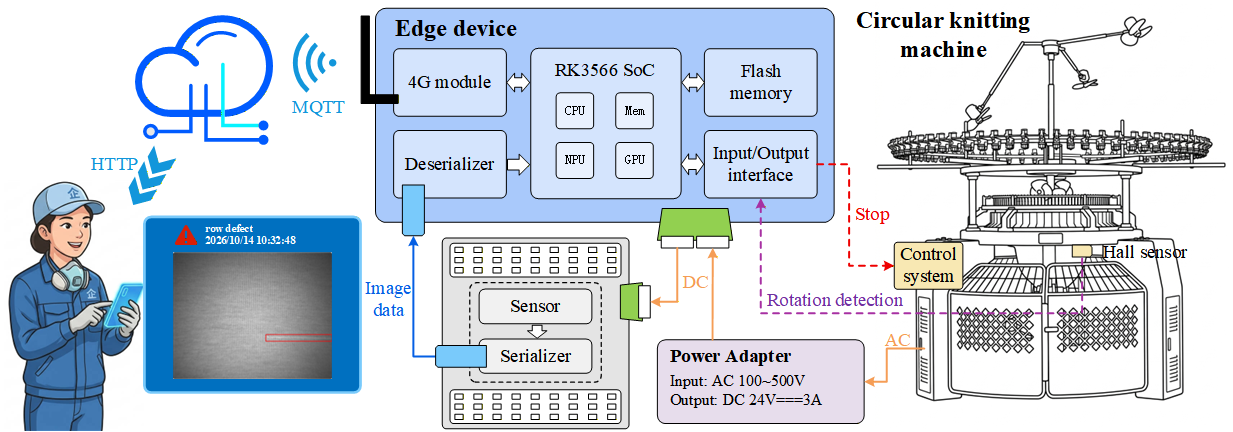
\includegraphics[width=0.92\textwidth]{fig1.png}
\caption{The device comprises LED illumination control, a coaxial image link to the RK3566, 4G cloud connectivity, and I/O for rotation sensing and machine control.}
\label{fig:interactions}
\end{figure*}

\subsection{Power Supply Subsystem}
To accommodate different industrial supply voltages across countries and regions, we design a power adapter with a 100--500 V AC input range and a 24 V DC output rated at 3 A. The adapter first supplies this output to the device. The device then supplies the LED illumination. By adjusting the current delivered to the LEDs, the device controls the illumination brightness to suit the image-acquisition conditions. This arrangement integrates LED power delivery and brightness control into the device.

\subsection{Image Acquisition and Transmission Subsystem}
The rapid rotation of circular knitting machines requires imaging that preserves defect geometry and fine spatial detail. We therefore select a SmartSens SC130GS global-shutter sensor (SmartSens Technology Co., Ltd., Shanghai, China) at $1280\times1024$ resolution, which exposes all pixels simultaneously to avoid motion-induced distortion from sequential row exposure. At a camera-to-fabric distance of approximately 10 cm, the field of view is approximately $16\times12$ cm, with the 16 cm dimension aligned with the horizontal direction of fabric motion.

Factory machinery creates an electromagnetically noisy environment, and installation requires the camera and edge device to be separated by a cable run. We therefore use serializer/deserializer (SerDes) transmission over shielded coaxial cable to accommodate remote camera placement and the interference environment. Specifically, the THCV241A serializer and THCV242A deserializer (THine Electronics, Inc., Tokyo, Japan) bridge the camera-side and processor-side MIPI CSI-2 interfaces. The link supports a maximum serial line rate of 4.0 Gb/s per lane, corresponding to a rated effective rate of 3.2 Gb/s \cite{thineTHCV241A,thineTHCV242A}.

The camera is configured to transmit $1280\times1024$ RAW10 images at 30 frames/s. With $b=10$ bits per pixel, the active-image payload rate is
\begin{equation}
\begin{aligned}
R_{\mathrm{img}} &= W H b f_{\mathrm{cam}} \\
&=1280\times1024\times10\times30 \\
&=393.216\ \mathrm{Mb/s}
\end{aligned}
\label{eq:serdes-bandwidth}
\end{equation}
\noindent where $W$ and $H$ denote the image width and height, and $f_{\mathrm{cam}}$ is the camera acquisition rate. This corresponds to only 12.3\% of the rated single-lane effective capacity, providing a stable image input for the detection system.

\subsection{Processor Subsystem}
\label{sec:coverage}
The processor is selected according to the detection rate required by fabric motion and the camera field of view. Taking a typical circular knitting machine as an example, with a machine diameter of 40 in ($D=1.016$ m) and a rotation period of $T=2$ s, the fabric travels approximately $\pi D=3.192$ m per revolution. With an effective field-of-view width of $w=0.16$ m along the direction of motion, the required frame rate is
\begin{equation}
f_{\min}=\frac{\pi D}{Tw}
=\frac{\pi\times1.016}{2\times0.16}
\approx9.97\ \mathrm{frames/s}
\label{eq:coverage-rate}
\end{equation}
\noindent We set the effective detection-throughput requirement to 10 frames/s. For this throughput target, we select the Rockchip RK3566 (Rockchip Electronics Co., Ltd., Fuzhou, China) to balance processing capability, camera connectivity, and hardware cost. It integrates a quad-core Cortex-A55 CPU and an NPU rated at 1 TOPS for INT8 operations \cite{rockchiprk3566}.

Table~\ref{tab:hardware-platforms} summarizes the hardware specifications of platforms used in related defect detection studies. While high-performance platforms like the NVIDIA Jetson Orin Nano and Xilinx ZCU102 offer substantial computational power, their costs range from hundreds to over 3,000 USD, which can be prohibitive for large-scale deployment. In contrast, our device provides a cost-effective hardware basis for the proposed system at a hardware cost of 60 USD, offering a significant cost advantage over comparable industrial platforms and making it highly suitable for large-scale deployment in textile factories.

\begin{table}[!tbp]
\caption{Hardware platforms used in related defect detection studies.}
\label{tab:hardware-platforms}
\centering
\footnotesize
\setlength{\tabcolsep}{3pt}
\renewcommand{\arraystretch}{1.0}
\begin{tabular}{@{}L{0.45\columnwidth}L{0.33\columnwidth}L{\dimexpr0.22\columnwidth-12pt\relax}@{}}
\toprule
Platform & Compute capability & Price (USD) \\
\midrule
NVIDIA Jetson TX2 NX\cite{li2024liteyolo} & 1.33 TFLOPS (FP16) & 249 \\
NVIDIA Jetson Xavier NX\cite{wang2024rail,zhang2026uavedge} & 21 TOPS (INT8) & 399 \\
NVIDIA Jetson Orin Nano\cite{machado2025edgefabric} & 40 TOPS (INT8) & 499 \\
Huawei Ascend 310\cite{yan2026warplace} & 16 TOPS (INT8) & 550 \\
AMD Xilinx ZCU102\cite{zhao2025kamnet} & 3.45 TOPS (INT8)\textsuperscript{\textdagger} & 3234 \\
Our device & 1 TOPS (INT8) & 60 \\
\bottomrule
\end{tabular}
\par\vspace{1pt}
\begin{minipage}{\columnwidth}
\footnotesize
\textsuperscript{\textdagger}AMD reference INT8 peak for three B4096 DPU cores.
\end{minipage}
\renewcommand{\arraystretch}{1.0}
\end{table}

\subsection{Hardware Implementation}
\label{sec:hardware-implementation}
Based on the design requirements of the subsystems described above, we develop the corresponding hardware shown in Fig.~\ref{fig:hardware}. The camera assembly (a) combines the image sensor and LED illumination. We design a camera-side interface board (b) that integrates the serializer and coaxial connector, and a mainboard (c) built around the RK3566. The mainboard integrates flash storage, the camera deserializer and coaxial connector, a 4G module with SIM-card and antenna interface, input/output interface, and power-management circuitry. This board-level integration brings image reception, local inference, network communication, machine control, and illumination control into a dedicated edge device. Fig.~\ref{fig:system} shows the system installed on a circular knitting machine in a real production line.

\begin{figure*}[!tbp]
\centering
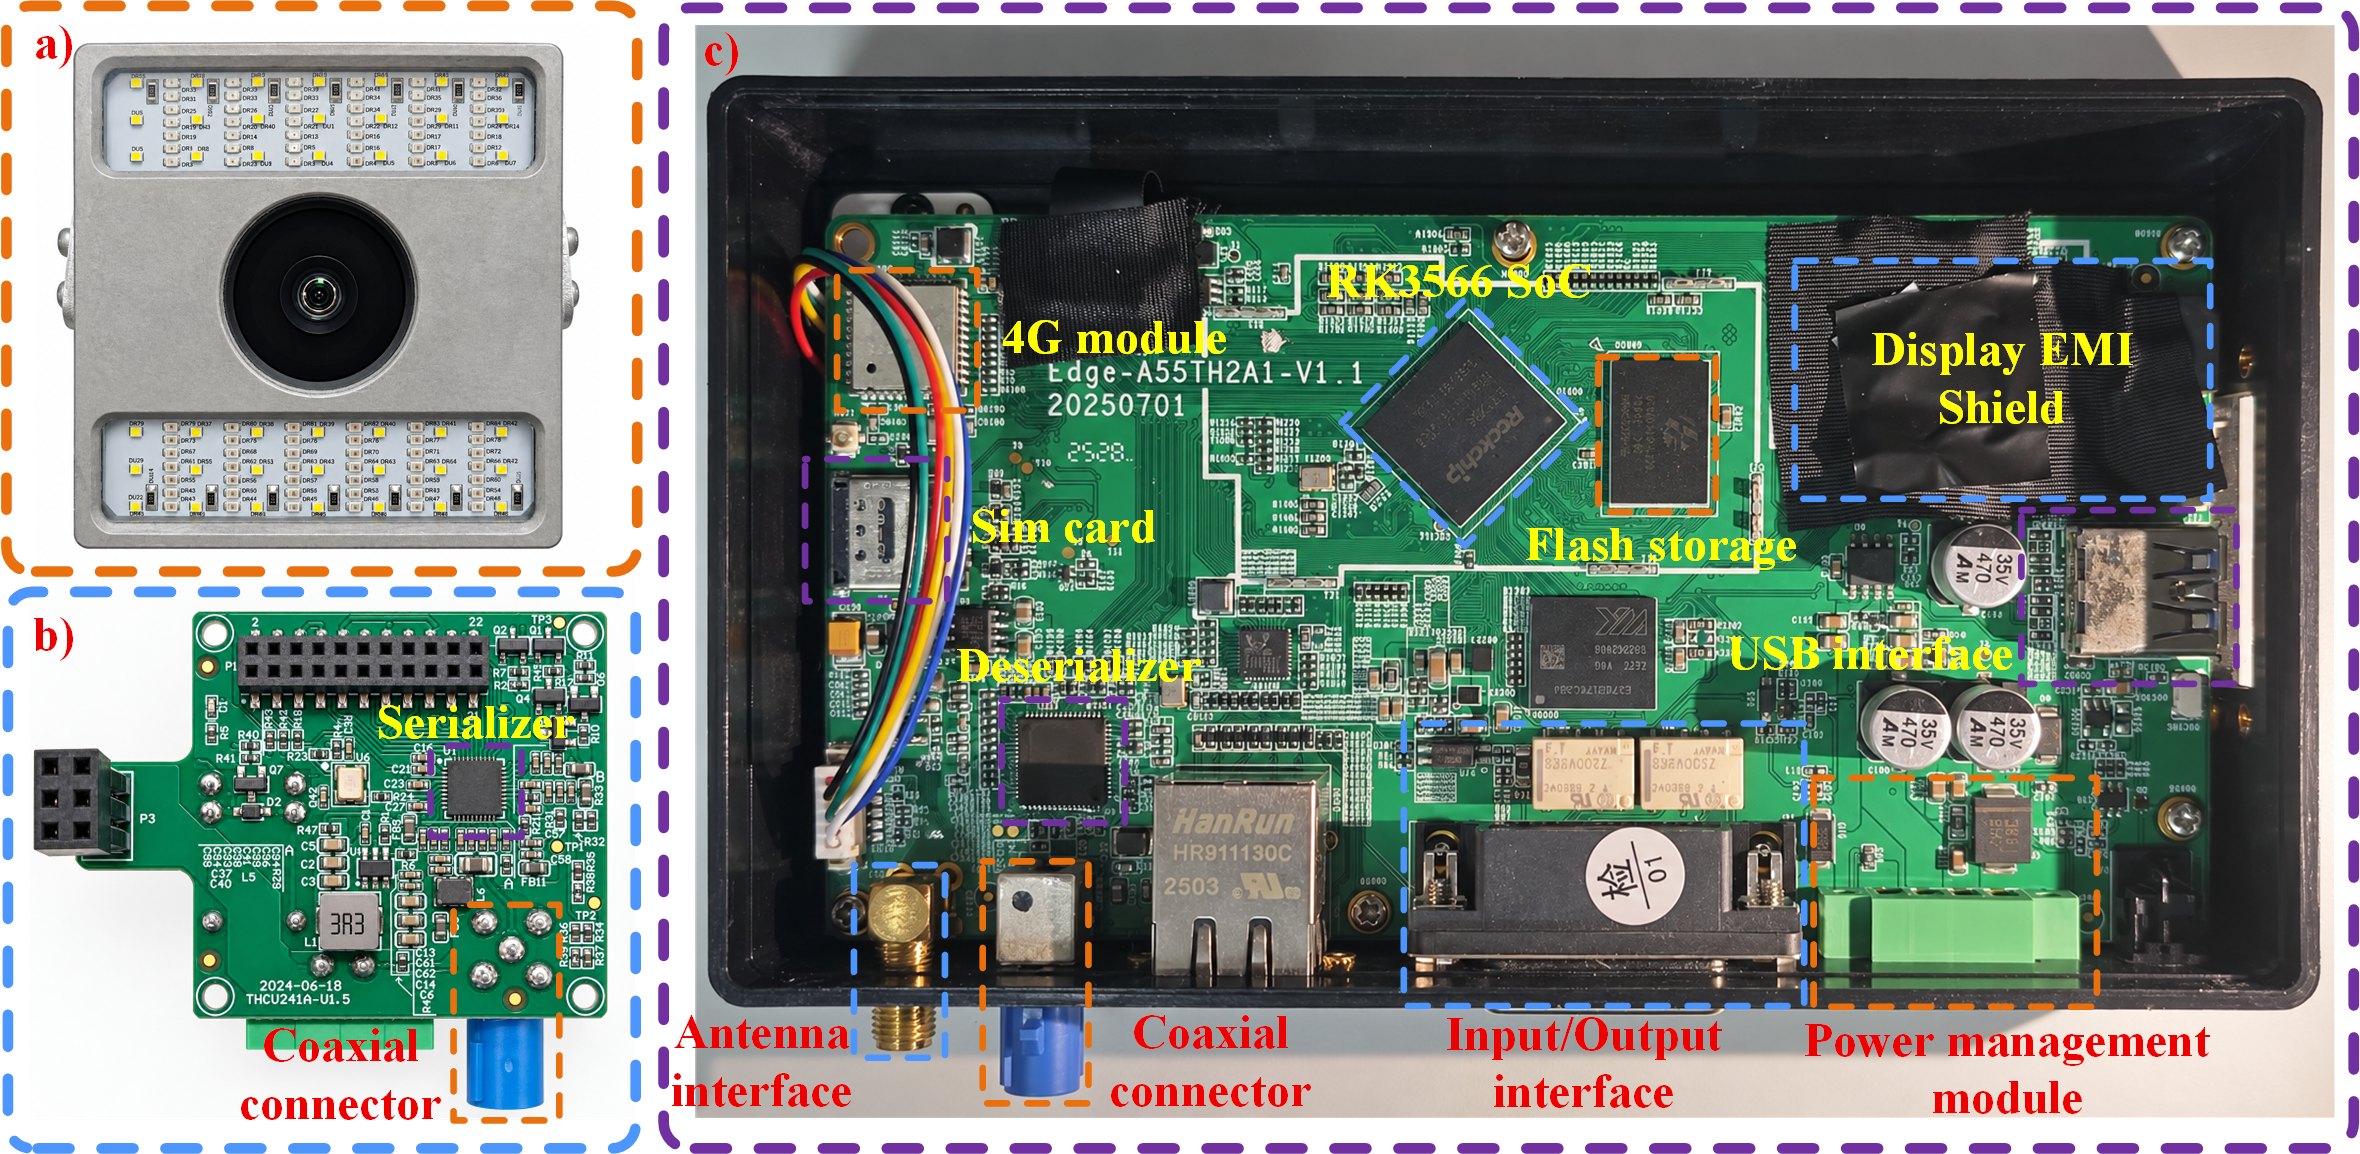
\includegraphics[width=0.86\textwidth]{fig2.png}
\caption{Hardware of the defect detection system: (a) industrial camera with LED illumination; (b) camera-side interface board with a serializer and coaxial connector; and (c) RK3566 edge board with the 4G communication, flash storage, camera-interface, input/output interface, and power-management components.}
\label{fig:hardware}
\end{figure*}

\begin{figure*}[!tbp]
\centering
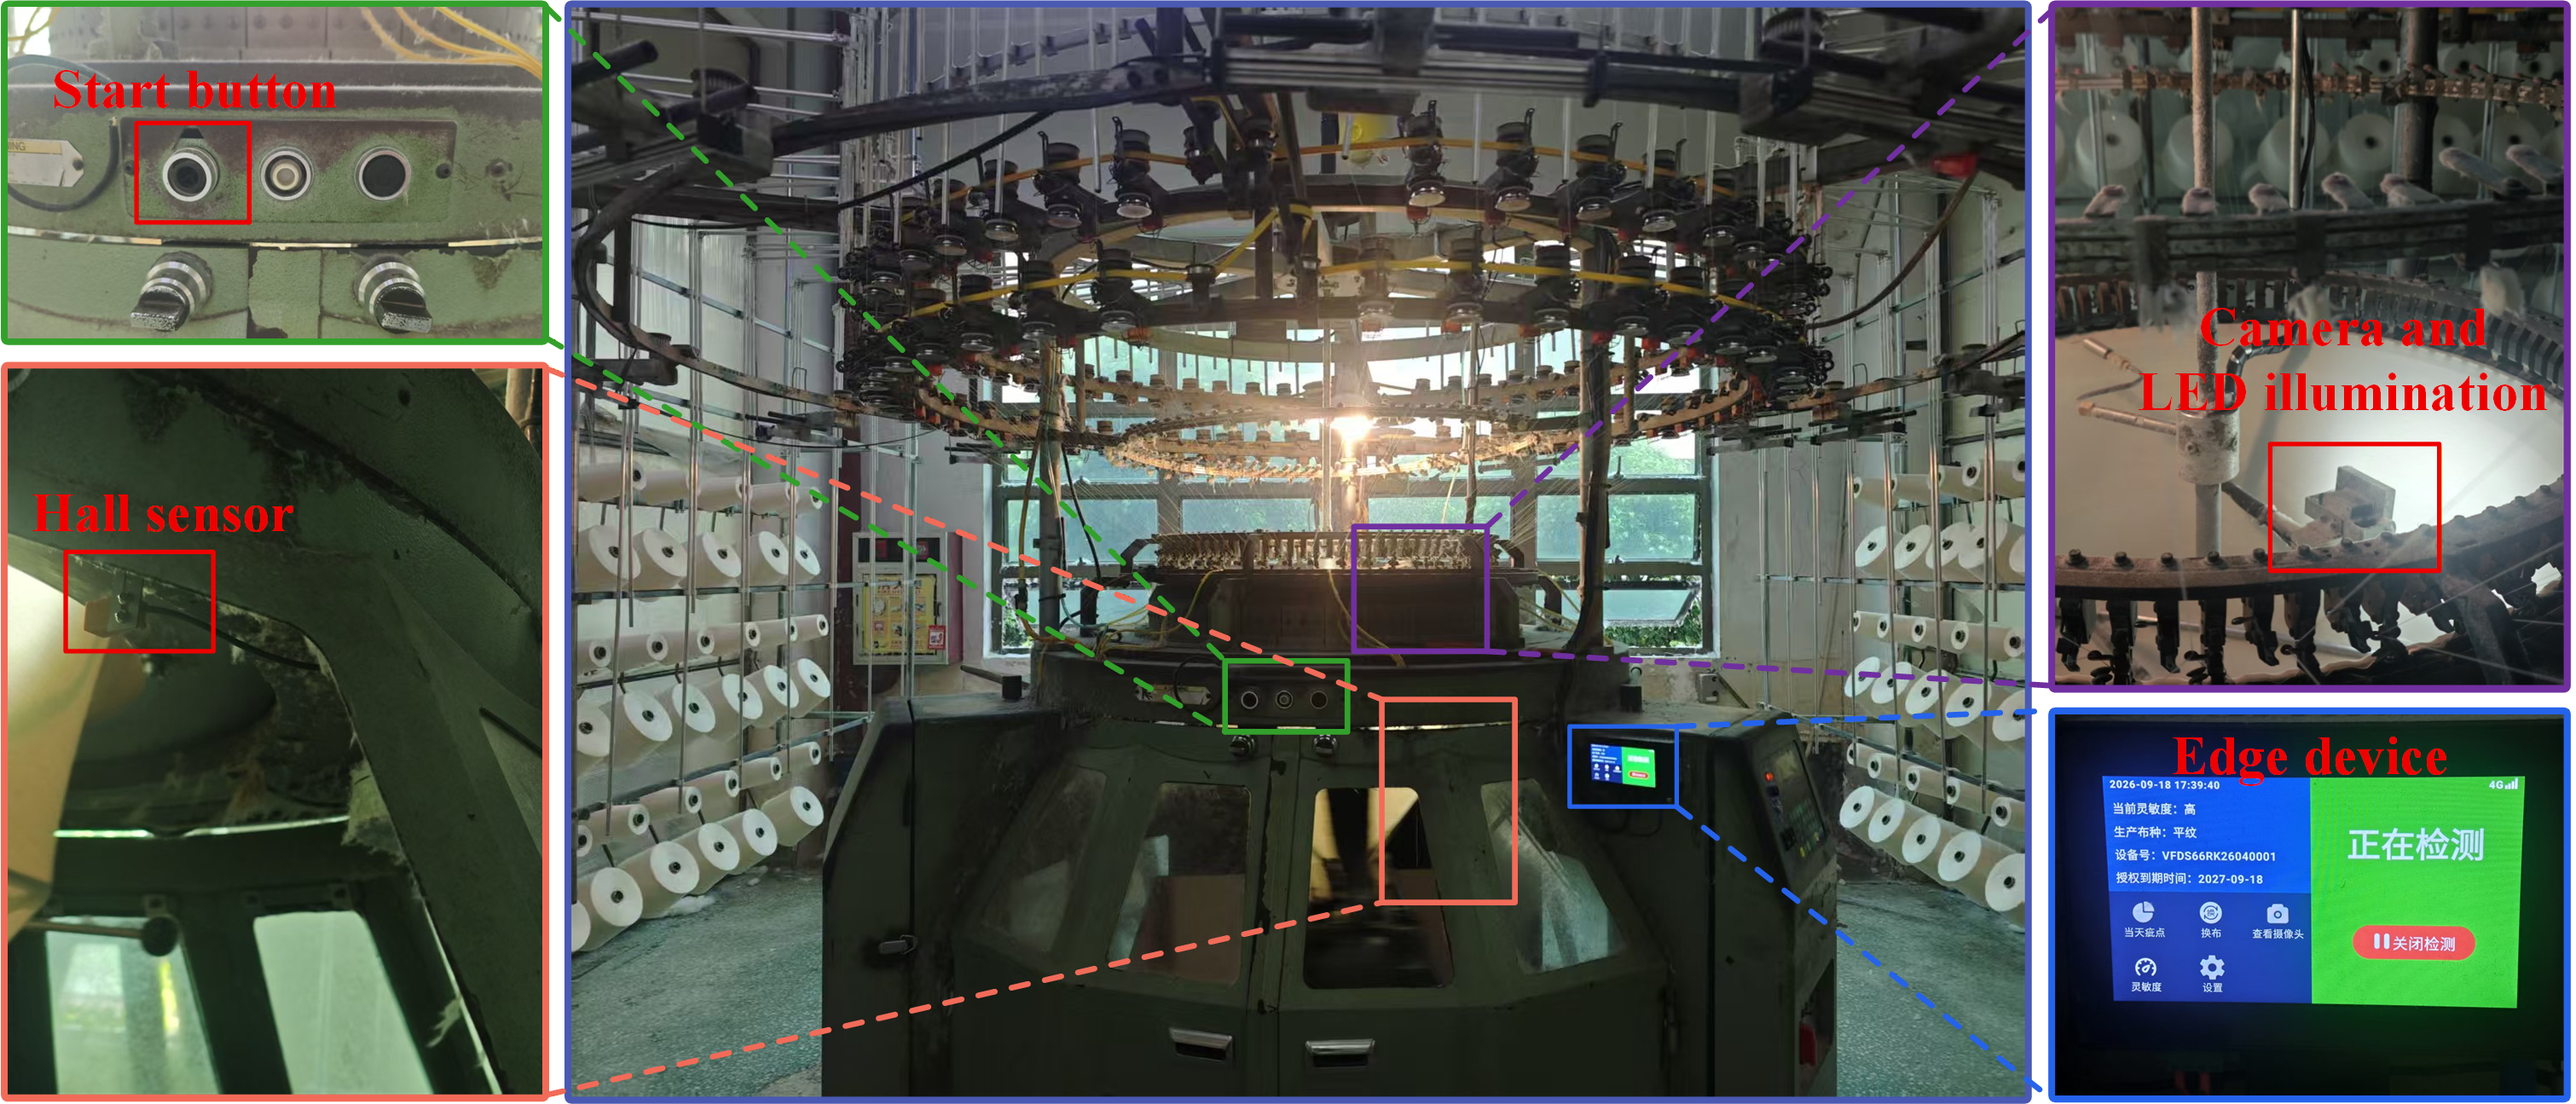
\includegraphics[width=0.86\textwidth]{fig3.png}
\caption{Actual deployment on the circular knitting machine at Dongguan Minghai Textile Co., Ltd., Dongguan, Guangdong, China. The insets highlight the start button, Hall sensor, industrial camera, and RK3566 edge device, respectively.}
\label{fig:system}
\end{figure*}

\section{Detection Algorithm}
\label{sec:method}
\subsection{Network Architecture}
Fig.~\ref{fig:network} shows the detector developed from YOLOv8n \cite{ultralytics2023}. Selective gradient residual enhancement (SGRE) is inserted after every bottleneck in the P3 and P4 backbone C2f blocks, progressively incorporating selected boundary responses while preserving the original feature paths. Subpixel-adaptive residual upsampling (SARU) replaces the two top-down upsampling operations, using content-dependent weights for the four output positions of each low-resolution cell. The remaining backbone stages, bottom-up aggregation path, and three-scale detection head are retained \cite{lin2017fpn,liu2018panet}.

\begin{figure*}[!tbp]
\centering
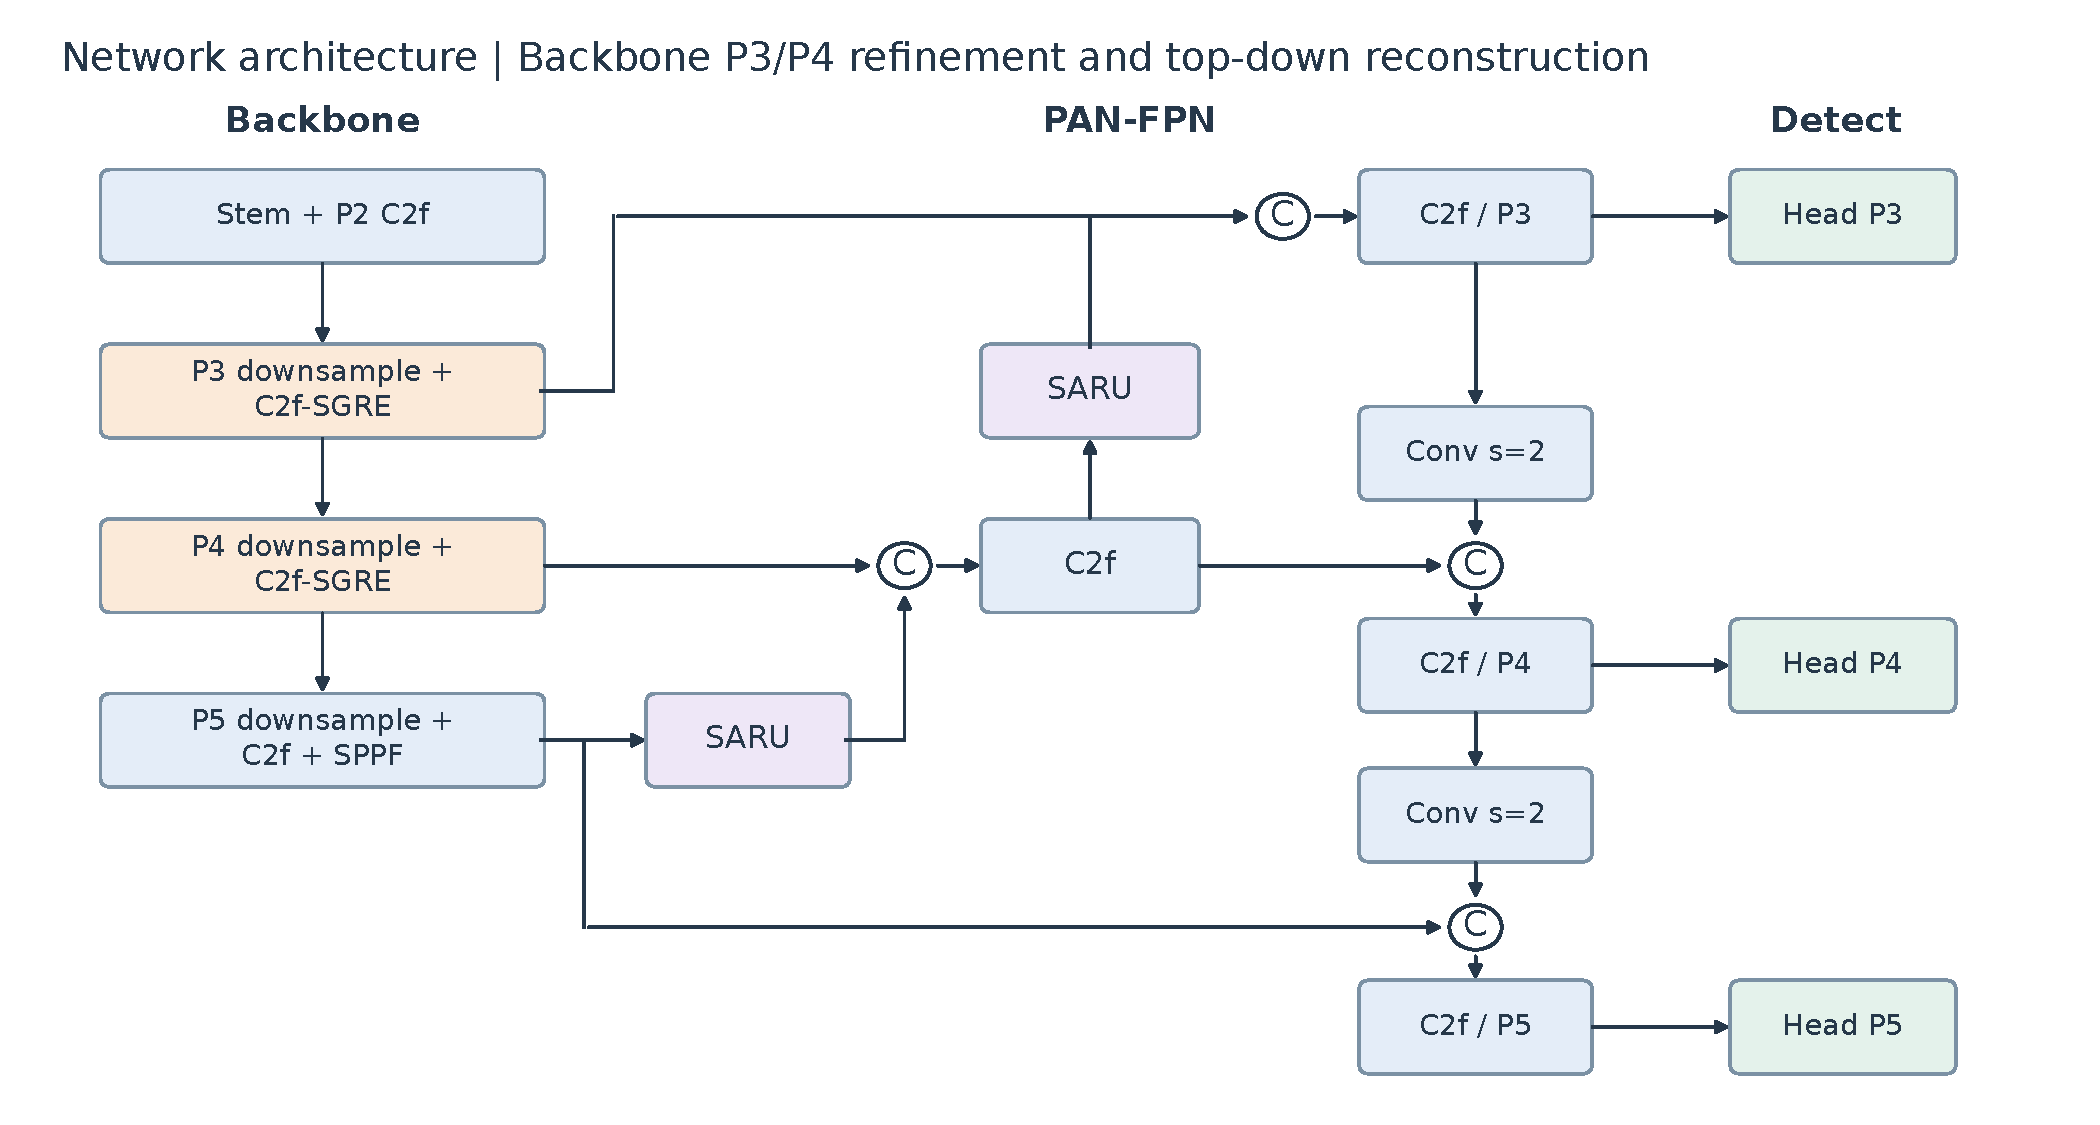
\includegraphics[width=0.95\textwidth]{network-v3.pdf}
\caption{Network architecture of the proposed detector. Each bottleneck in the backbone P3 and P4 C2f blocks is followed by SGRE. SARU replaces the two top-down upsampling operations. C denotes channel concatenation; downsampling convolutions and the three-scale detection head retain the YOLOv8n structure.}
\label{fig:network}
\end{figure*}

\subsection{Selective Gradient Residual Enhancement}
Knitting defects can produce narrow, weak boundaries against repetitive fabric texture. Their boundary responses provide complementary evidence to the features learned by convolution, but gradient magnitude alone also responds to normal yarn patterns. We therefore develop SGRE to select and mix gradient evidence before adding it to the original features [Fig.~\ref{fig:modules}(a)]. The Sobel filters supply a fixed local derivative prior, whereas the selection and channel mixing are learned from the detection objective. SGRE is applied to all hidden channels after each complete bottleneck output, including its original shortcut, in the backbone P3 and P4 C2f blocks. This placement lets the enhanced output enter both the next bottleneck and the final C2f concatenation. P2 and P5 retain their original C2f blocks.

\emph{1) Fixed Gradient Extraction:}
For a bottleneck output $F\in\mathbb{R}^{B\times C\times H\times W}$, two depthwise convolutions compute gradients using normalized Sobel kernels:
\begin{equation}
K_x=\frac{1}{8}\begin{bmatrix}-1&0&1\\-2&0&2\\-1&0&1\end{bmatrix}
\qquad K_y=K_x^{\mathsf T}
\label{eq:sgre-kernels}
\end{equation}
\noindent The gradient evidence is formed as
\begin{equation}
E=\left|K_x*_{\mathrm{dw}}F\right|+\left|K_y*_{\mathrm{dw}}F\right|
\label{eq:sgre-gradient}
\end{equation}
\noindent where $*_{\mathrm{dw}}$ denotes channel-independent convolution with padding of one. Both absolute-value operations are performed before summation. Thus $E$ has the same $B\times C\times H\times W$ shape as $F$. The two Sobel kernels remain fixed during training.

\emph{2) Selective Residual Enhancement:}
A learned depthwise convolution and Hardsigmoid predict channel-specific spatial selection weights from the original feature, while a separate pointwise convolution mixes the gradient evidence:
\begin{align}
G &= \operatorname{HS}(\operatorname{DWConv}_{3\times3}(F))
\label{eq:sgre-selection}\\
R &= \operatorname{Conv}_{1\times1}(E)
\label{eq:sgre-projection}\\
Z &= F+G\odot R
\label{eq:sgre-output}
\end{align}
\noindent where $G,R,Z\in\mathbb{R}^{B\times C\times H\times W}$. The depthwise selection convolution includes a bias, whereas the $C$-to-$C$ pointwise projection is bias-free. The selection weights regulate the contribution of gradient evidence at each channel and spatial position, and the residual connection retains the original feature. There is no partial-channel split inside SGRE. The selection convolution and pointwise projection are initialized to zero, giving $G=0.5$ and $Z=F$ at initialization.

For a selected C2f block, let $U,V$ denote its two initial hidden branches. The enhanced progressive outputs satisfy
\begin{equation}
Z_0=V\qquad
Z_i=\operatorname{SGRE}_i(\operatorname{Bottleneck}_i(Z_{i-1}))
\label{eq:sgre-progressive}
\end{equation}
\noindent for $i=1,\ldots,n$. The original C2f fusion concatenates $U$, $V$, and all enhanced outputs $Z_1,\ldots,Z_n$. Each SGRE has independent learned weights. Under the YOLOv8n scaling used here, P3 and P4 each contain two such bottlenecks, giving four SGRE units in total.

\emph{3) Computational Cost:}
For one SGRE with $C$ hidden channels, the added parameter count and convolutional MAC count are
\begin{align}
P_{\mathrm{SGRE}} &= C^2+10C
\label{eq:sgre-params}\\
\operatorname{MAC}_{\mathrm{SGRE}} &= BHW(C^2+27C)
\label{eq:sgre-macs}
\end{align}
\noindent The $C^2$ parameters belong to the pointwise projection; the depthwise selector contributes $9C$ weights and $C$ biases. The fixed Sobel filters are stored as buffers rather than model parameters. In convolutional computation, however, both filters still contribute $18C$ MACs per spatial location, in addition to the selector's $9C$ and the projection's $C^2$ MACs. Absolute values, Hardsigmoid, and element-wise arithmetic introduce additional linear cost in $BCHW$. The complete added cost is obtained by summing over the four inserted units.

\begin{figure*}[!tbp]
\centering
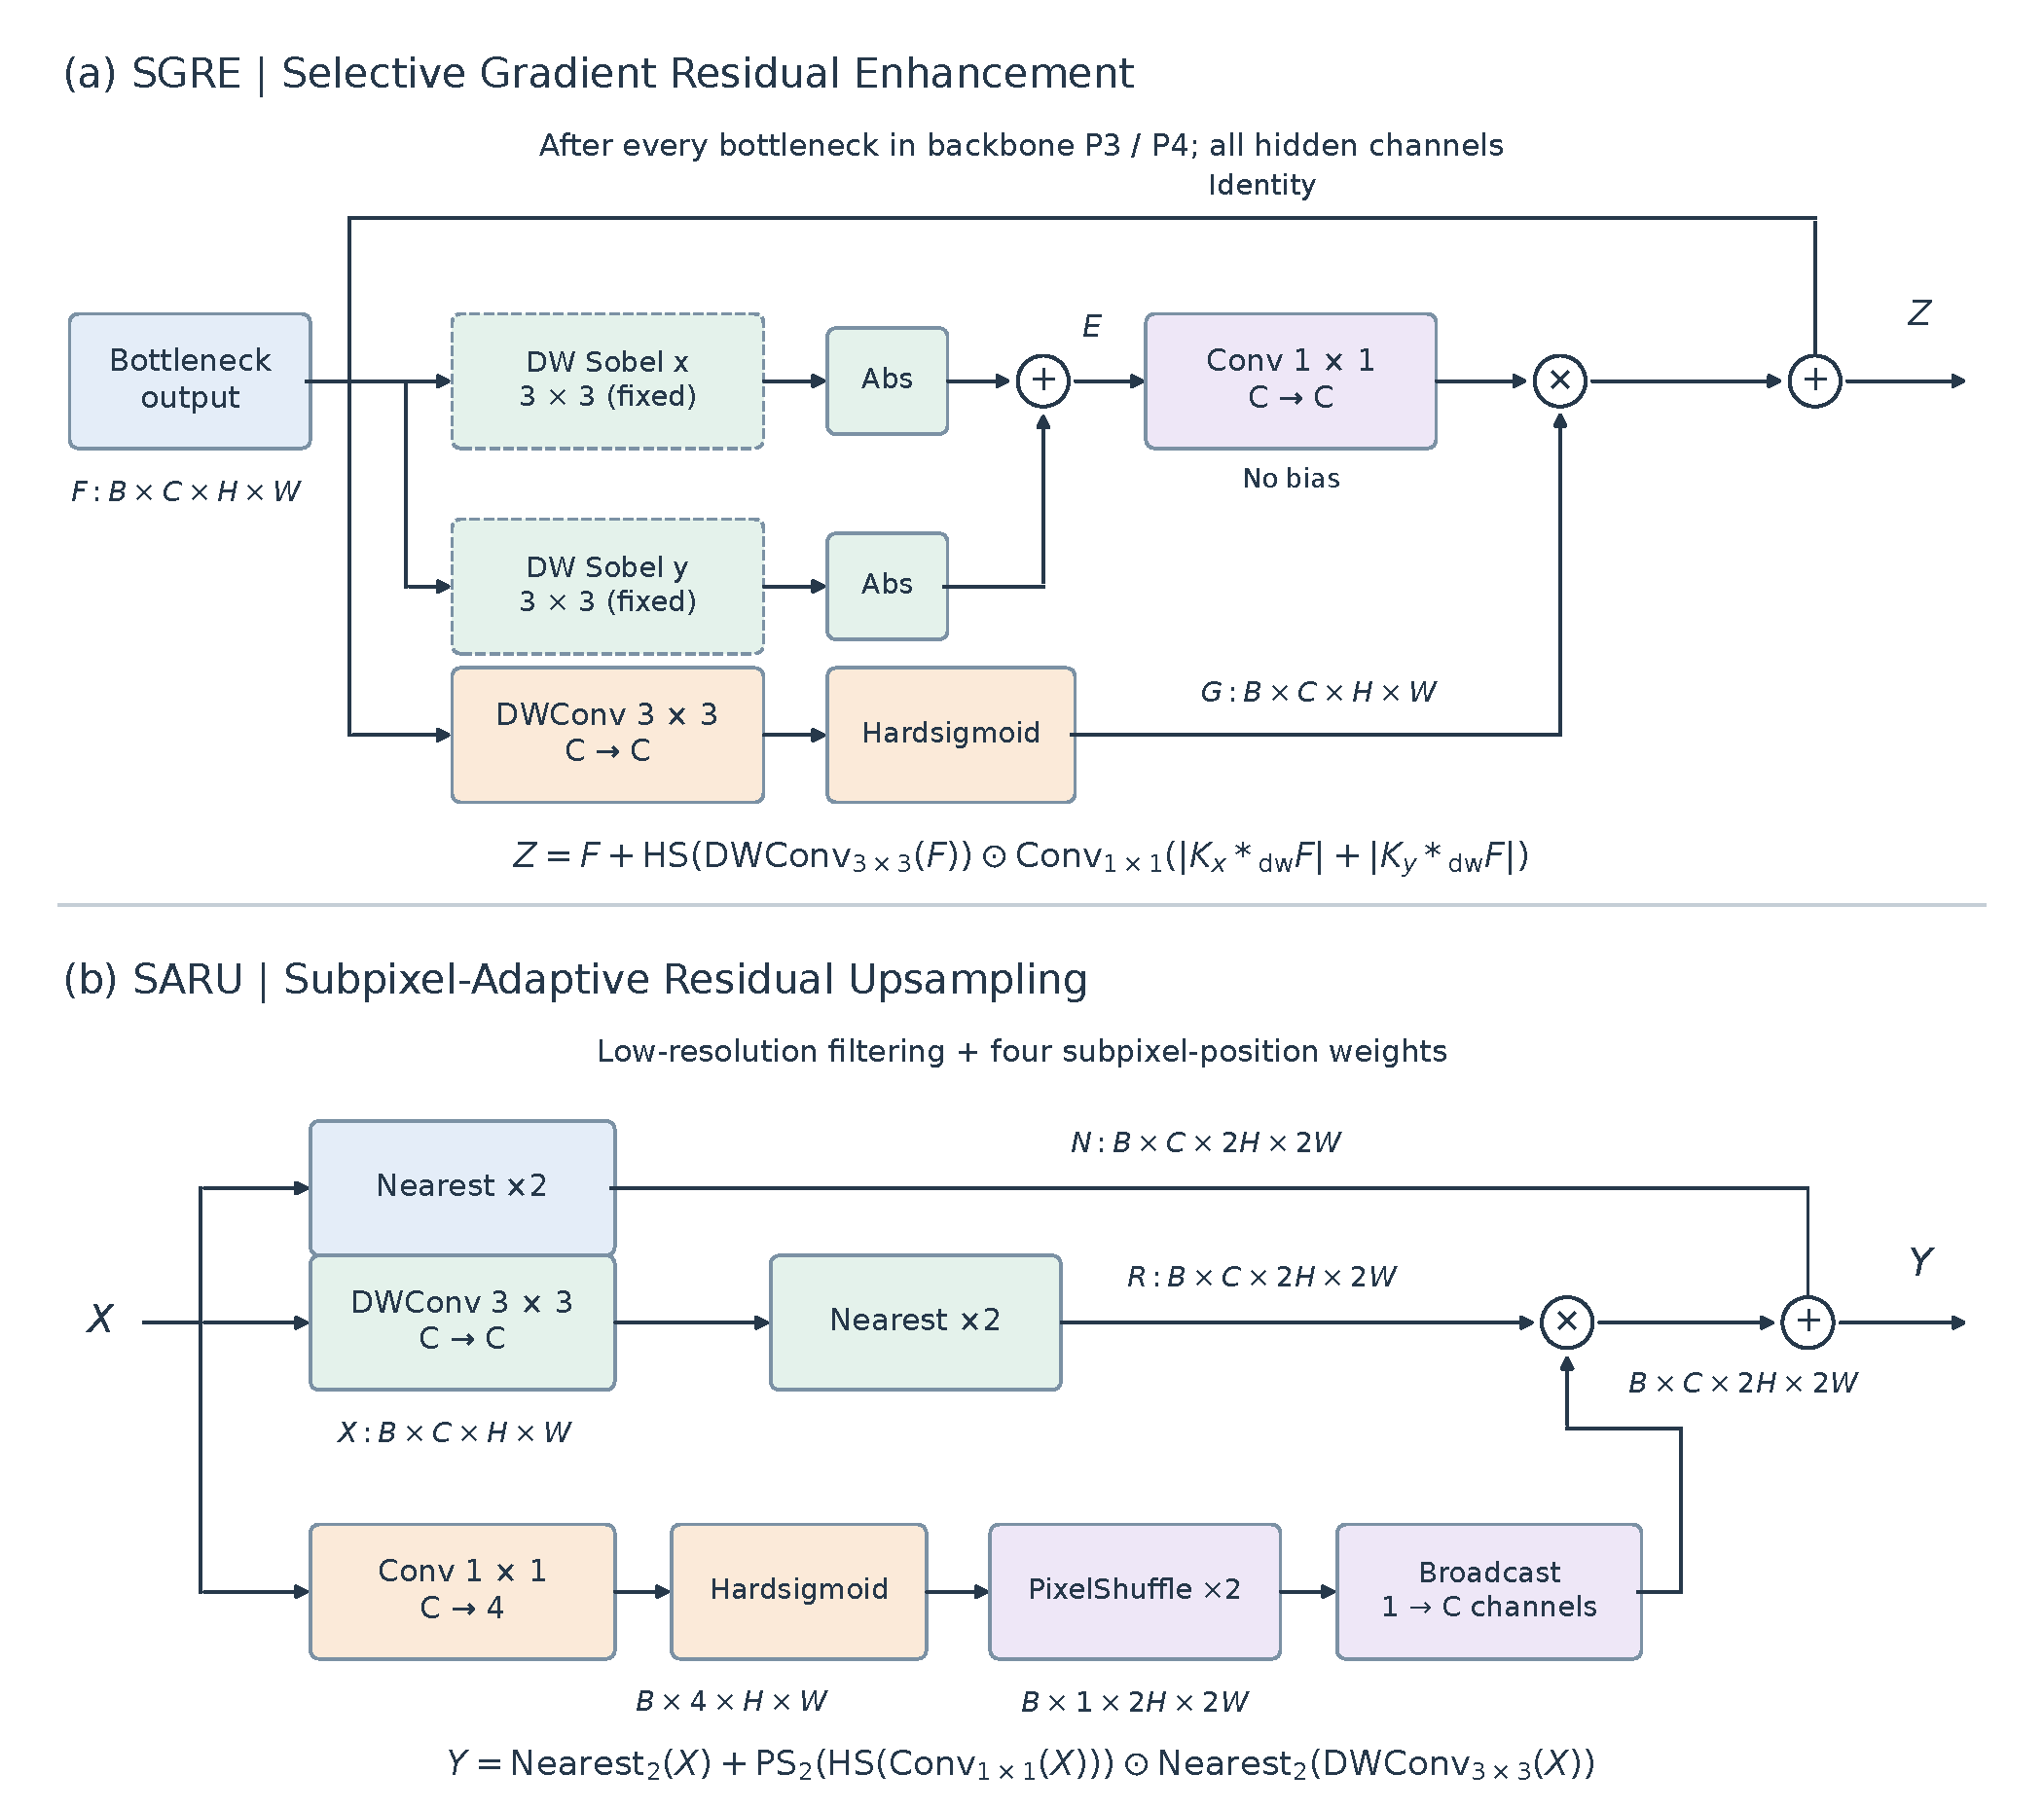
\includegraphics[width=\textwidth]{modules-v3.pdf}
\caption{Implementation-matched module structures: (a) SGRE applies fixed depthwise Sobel filters, channel-wise spatial selection, and learned pointwise mixing to a complete bottleneck output; (b) SARU adds a low-resolution filtered residual to nearest-neighbor upsampling. PixelShuffle rearranges four weights into four distinct subpixel positions; the resulting single-channel map is broadcast across feature channels before multiplication. Dashed blocks denote fixed filters.}
\label{fig:modules}
\end{figure*}

\subsection{Subpixel-Adaptive Residual Upsampling}
In the top-down feature pyramid, a low-resolution cell is expanded into four output positions before fusion with lateral features. These positions can cover different parts of a narrow defect or a hole boundary. Nearest-neighbor interpolation assigns the same response to all four positions and does not allow their reconstruction to depend on local content. SARU retains this parameter-free base and adds a locally filtered residual with separate content-dependent weights for the four subpixel positions [Fig.~\ref{fig:modules}(b)]. The learned filtering and weight prediction operate at the low resolution to limit computation. Unlike a four-channel feature expansion, the four predicted channels encode positional weights shared across feature channels.

\emph{1) Base and Residual Paths:}
For $X\in\mathbb{R}^{B\times C\times H\times W}$, the two feature paths are
\begin{align}
N &= \operatorname{Nearest}_{2}(X)
\label{eq:saru-base}\\
R &= \operatorname{Nearest}_{2}(\operatorname{DWConv}_{3\times3}(X))
\label{eq:saru-residual}
\end{align}
\noindent where $N,R\in\mathbb{R}^{B\times C\times2H\times2W}$. The residual convolution is depthwise, bias-free, and uses padding of one. It filters neighboring low-resolution responses before expansion, whereas $N$ preserves the baseline nearest-neighbor feature.

\emph{2) Subpixel Weight Prediction:}
A biased pointwise convolution maps $C$ channels to four position-dependent weights, which are rearranged by PixelShuffle:
\begin{align}
A &= \operatorname{HS}(\operatorname{Conv}^{C\rightarrow4}_{1\times1}(X))
\label{eq:saru-weights}\\
G &= \operatorname{PixelShuffle}_{2}(A)
\label{eq:saru-shuffle}
\end{align}
\noindent Here, $A\in[0,1]^{B\times4\times H\times W}$ and $G\in[0,1]^{B\times1\times2H\times2W}$. For zero-based spatial indices $h,w$ and offsets $i,j\in\{0,1\}$, the rearrangement is
\begin{equation}
G(b,1,2h+i,2w+j)=A(b,2i+j+1,h,w)
\label{eq:saru-positions}
\end{equation}
\noindent so the four predicted channels correspond to the top-left, top-right, bottom-left, and bottom-right positions. Before multiplication, $G$ is broadcast along the channel dimension from $B\times1\times2H\times2W$ to $B\times C\times2H\times2W$ by reusing the same spatial weights for all $C$ channels.

\emph{3) Residual Reconstruction and Cost:}
The reconstructed feature is
\begin{equation}
Y=N+G\odot R
\label{eq:saru-output}
\end{equation}
\noindent where the multiplication uses channel broadcasting and $Y\in\mathbb{R}^{B\times C\times2H\times2W}$. This additive correction can increase or decrease a feature response because $R$ is signed. Zero-initializing the depthwise residual convolution and the four-output predictor makes $R=0$, $G=0.5$, and $Y=N$ at initialization.

The added parameter and convolutional MAC counts are
\begin{align}
P_{\mathrm{SARU}} &= 13C+4
\label{eq:saru-params}\\
\operatorname{MAC}_{\mathrm{SARU}} &= 13BCHW
\label{eq:saru-macs}
\end{align}
\noindent The residual depthwise convolution contributes $9C$ weights, and the $C$-to-four predictor contributes $4C$ weights and four biases. Both convolutions operate at $H\times W$; PixelShuffle only rearranges weights, while nearest-neighbor interpolation copies values. The output multiplication and addition each operate on $4BCHW$ elements. Consequently, learned convolutional computation scales linearly with channel count without constructing a channel-by-neighborhood reassembly tensor. When expressing convolutional computation as FLOPs, one MAC is counted as two operations; these analytic convolution counts are separate from the full-model profiler totals.

\section{Experimental Setup}
\label{sec:experimental-setup}
\subsection{Dataset}
The dataset was collected from a real circular-knitting production line and covers three defect categories: horizontal defects (\emph{row}), vertical defects (\emph{col}), and holes (\emph{hole}). It comprises 403 images with 468 annotated defect instances, divided into training, validation, and test sets of 282, 40, and 81 images, respectively, as summarized in Table~\ref{tab:data}.
\begin{table}[!htbp]
\caption{Image-level split and defect-instance counts in the real production-line dataset.}
\label{tab:data}
\centering
\footnotesize
\begin{tabular}{lrrrrr}
\toprule
Split & Images & Instances & Row & Col & Hole \\
\midrule
Train & 282 & 329 & 174 & 75 & 80 \\
Validation & 40 & 48 & 24 & 13 & 11 \\
Test & 81 & 91 & 60 & 12 & 19 \\
\bottomrule
\end{tabular}
\end{table}

\subsection{Implementation Details}
\label{sec:implementation}
\begin{table}[!htbp]
\caption{Implementation protocol covering training (Ultralytics) and deployment (edge device).}
\label{tab:implementation}
\centering
\footnotesize
\setlength{\tabcolsep}{3pt}
\renewcommand{\arraystretch}{1.08}
\begin{tabular}{@{}L{0.21\columnwidth}L{0.23\columnwidth}L{\dimexpr0.56\columnwidth-12pt\relax}@{}}
\toprule
Category & Parameter & Specification \\
\midrule
\multirow[t]{2}{0.21\columnwidth}{Training setup}
& Hardware & Intel i7-13700KF; NVIDIA RTX 3090 (24 GB) \\
& Software & Ubuntu 24.04, Python 3.10.20, PyTorch 2.4.1+cu124, and Ultralytics 8.4.140 \\
\midrule
\multirow[t]{3}{0.21\columnwidth}{Deployment setup}
& Hardware & Rockchip RK3566 \\
& System & Android 13 \\
& Quantization & INT8 \\
\midrule
Data protocol
& Input resolution & Fixed at $640\times640$ \\
\midrule
\multirow[t]{4}{0.21\columnwidth}{Training dynamics}
& Batch & 16  \\
& Maximum epochs & 300 \\
& Patience & 80 epochs \\
& Optimizer & AdamW \\
\bottomrule
\end{tabular}
\renewcommand{\arraystretch}{1.0}
\end{table}

\begin{table*}[!tbp]
\caption{Detector comparison on the test set. FPS denotes FP32 model-forward throughput on an RTX 3090 with batch size 1 and a $640\times640$ input. Bold and underlined values indicate the best and second-best results, respectively.}
\label{tab:comparison}
\centering
\small
\setlength{\tabcolsep}{6pt}
\renewcommand{\arraystretch}{1.06}
\begin{tabular*}{\textwidth}{@{\extracolsep{\fill}}lrrrrr}
\toprule
Model & Params (M) & FLOPs (G) & mAP50 (\%) & mAP50--95 (\%) & FPS \\
\midrule
YOLOv9t~\cite{wang2025yolov9} & \textbf{2.12} & 8.5 & 90.1 & 53.3 & 291 \\
YOLOv10n~\cite{wang2024yolov10} & 2.78 & 8.8 & 88.2 & 58.5 & \underline{524} \\
YOLO11n~\cite{ultralytics2023} & 2.62 & \underline{6.7} & 93.3 & 60.8 & 463 \\
YOLO12n~\cite{tian2025yolov12} & 2.60 & 7.6 & 89.0 & 56.8 & 326 \\
YOLO26n~\cite{ultralytics2023} & \underline{2.57} & \textbf{6.2} & 90.5 & 58.2 & 425 \\
RT-DETR-R18~\cite{zhao2024rtdetr} & 20.09 & 60.7 & 95.2 & \textbf{67.7} & 146 \\
DETR-R50~\cite{carion2020detr} & 41.28 & 77.3 & 96.4 & 53.6 & 101 \\
Deformable DETR-R50~\cite{zhu2021deformable} & 39.8 & 158.7 & \underline{96.8} & 64.3 & 49 \\
Faster R-CNN-R50~\cite{ren2015faster} & 41.1 & 181.5 & 96.1 & 64.7 & 66 \\
YOLOv8n (Baseline)~\cite{ultralytics2023} & 3.01 & 8.1 & 90.5 & 58.4 & \textbf{554} \\
\model & 3.02 & 8.2 & \textbf{97.4} & \underline{65.5} & 491 \\
\bottomrule
\end{tabular*}
\par\smallskip
\renewcommand{\arraystretch}{1.0}
\end{table*}

\begin{figure*}[!tbp]
\centering
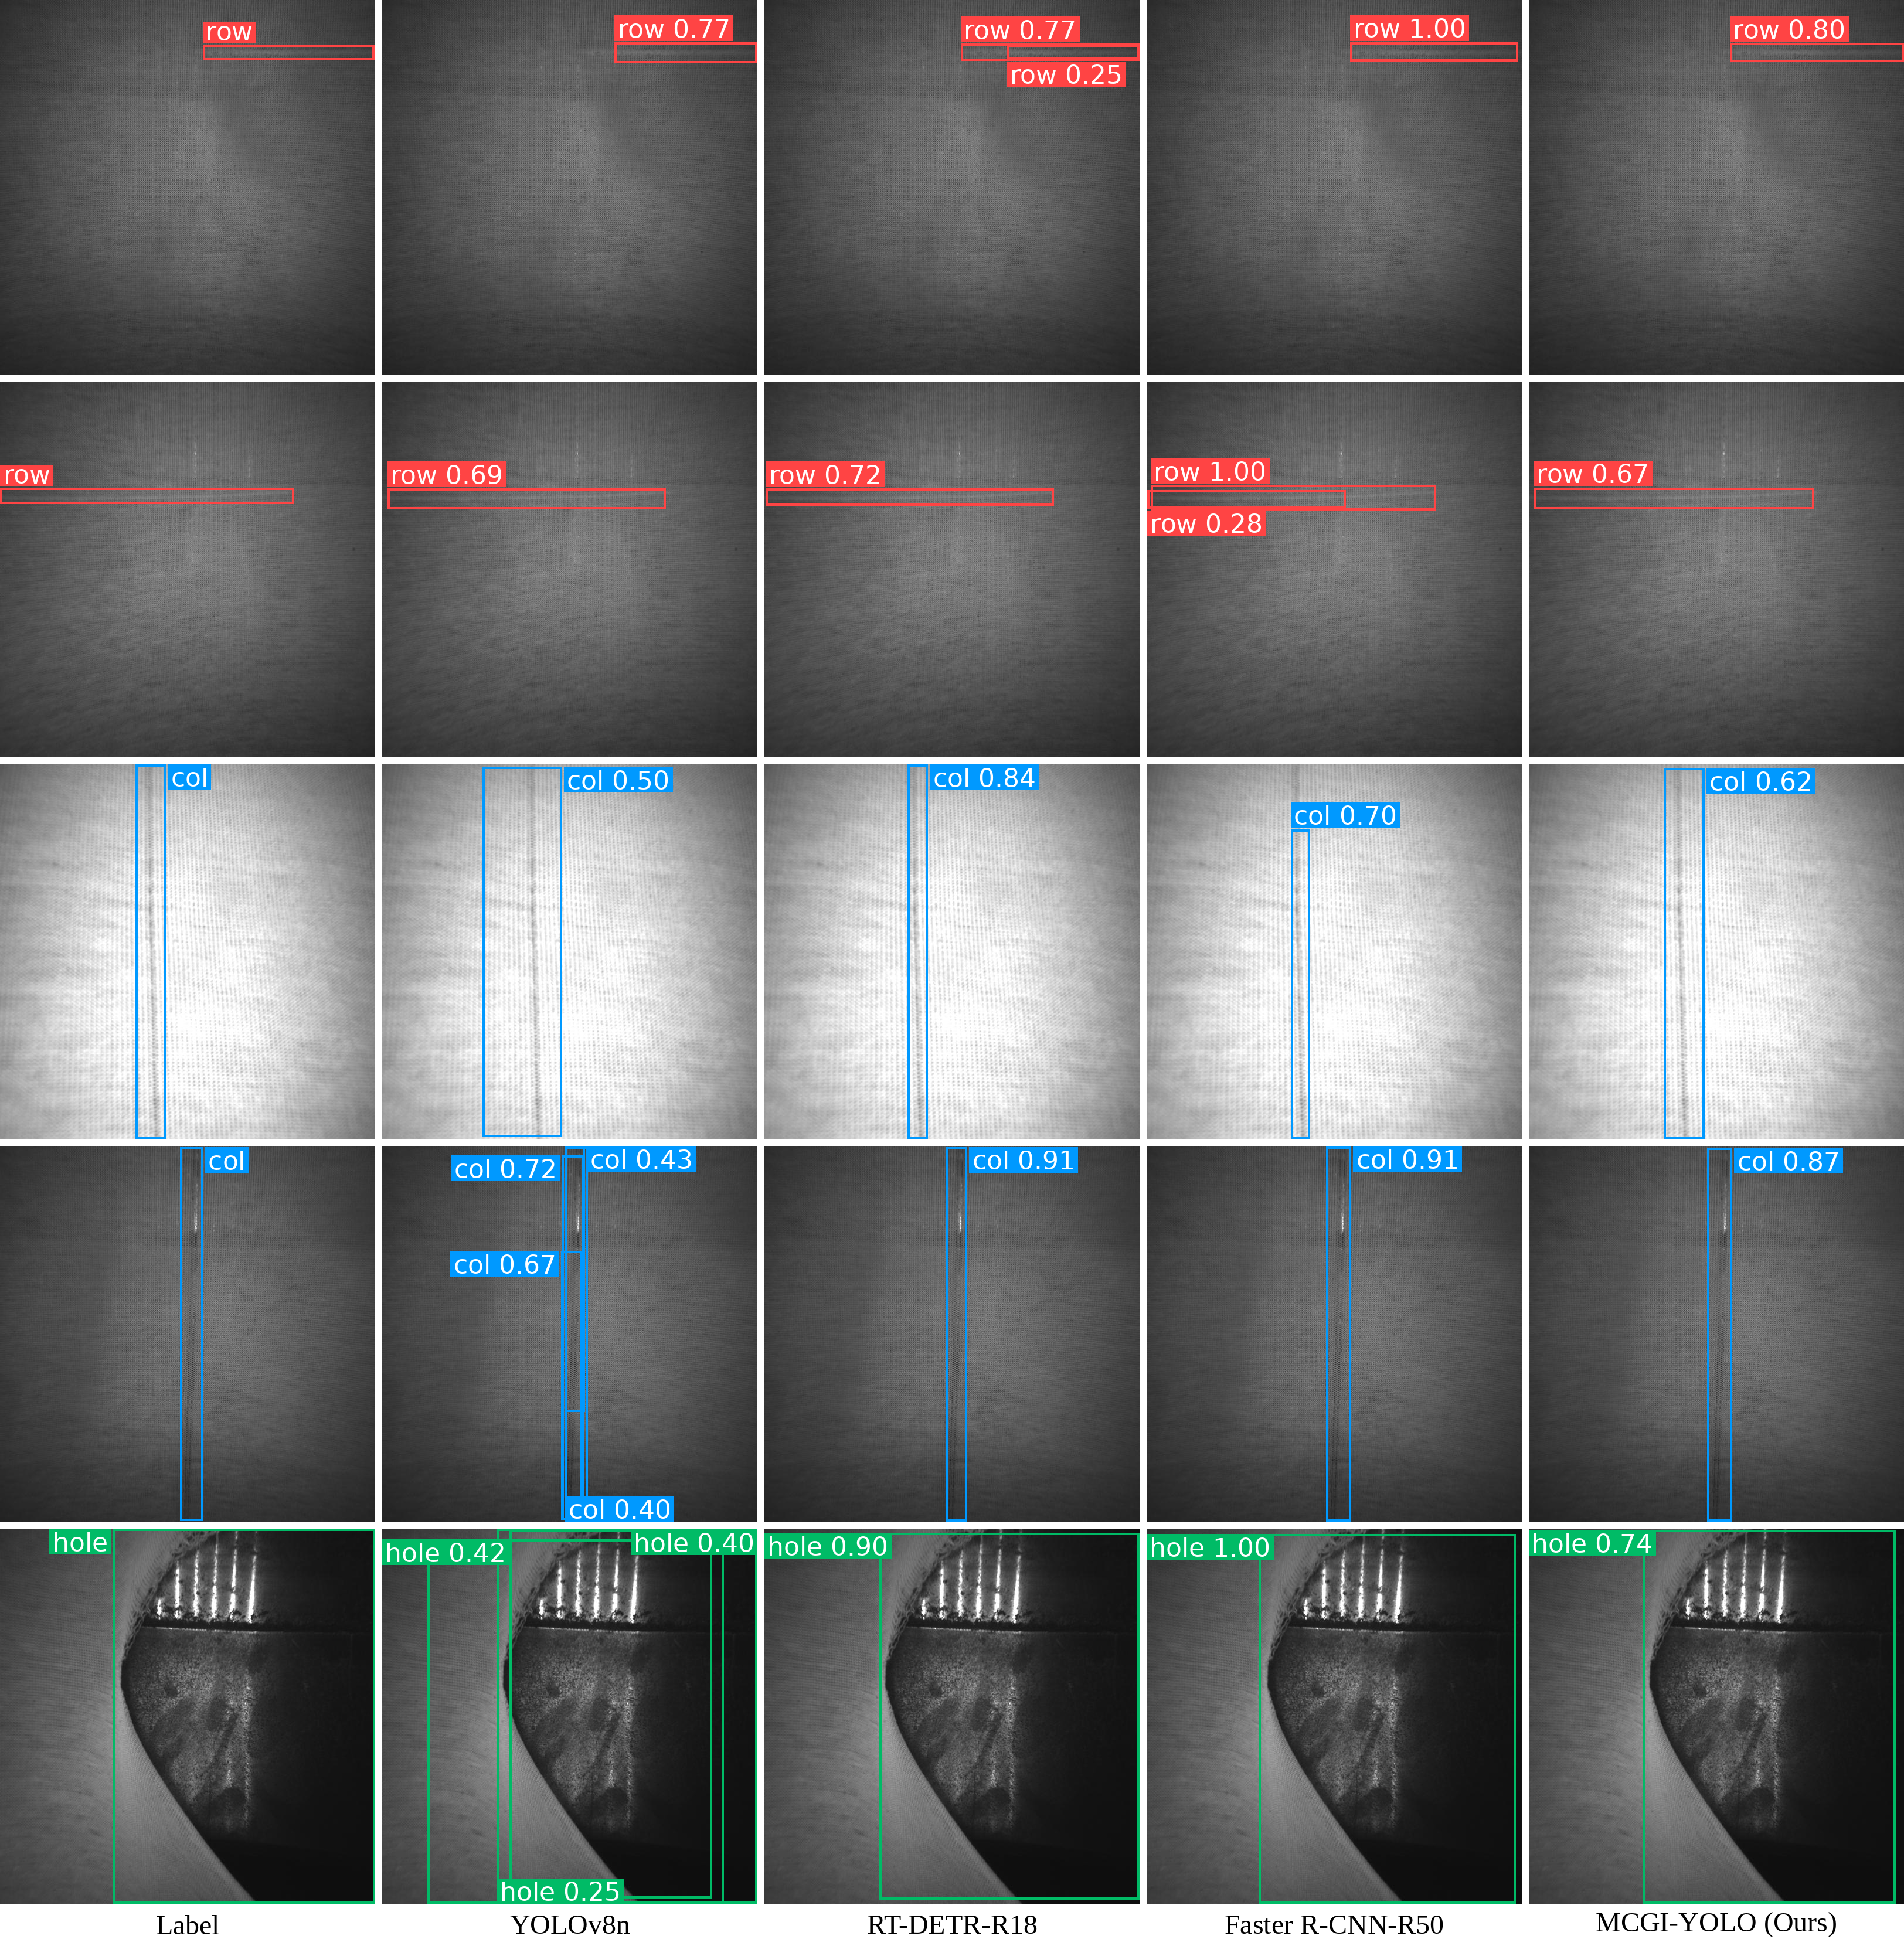
\includegraphics[width=0.86\textwidth]{fig6.png}
\caption{Qualitative comparison of detection results across different methods. From left to right: ground-truth annotations (Label), YOLOv8n, RT-DETR-R18, Faster R-CNN-R50, and \model (Ours).}
\label{fig:qualitative}
\end{figure*}

Table~\ref{tab:implementation} summarizes the training and deployment settings. \model and its component-ablation variants share the same \texttt{yolov8n.pt} initialization as the YOLOv8n baseline, and all component comparisons use a common training protocol with matched random seeds. Other comparison models use available pretrained checkpoints from their respective implementations.

\subsection{Evaluation Metrics}
\label{sec:evaluation}
Intersection over union (IoU) measures the overlap between predicted and ground-truth bounding boxes as the ratio of their intersection area to their union area. Detection accuracy is evaluated using mAP50 and mAP50--95. Let $a_c(t)$ denote the average precision for class $c$ at IoU threshold $t$. The metrics are computed as
\begin{align}
\operatorname{mAP}_{50} &= \frac{1}{N_c}\sum_{c=1}^{N_c}a_c(0.50)
\label{eq:metrics}\displaybreak[1]\\
\operatorname{mAP}_{50:95} &= \frac{1}{10N_c}\sum_{c=1}^{N_c}\sum_{t\in T}a_c(t)
\label{eq:ap}
\end{align}
\noindent where $N_c=3$ and $T=\{0.50,0.55,\ldots,0.95\}$. Both metrics are reported as percentages, with improvements expressed in percentage points.

Model parameters and FLOPs are measured at $640\times640$ input resolution using each model's respective framework. For FPS comparison, all models are evaluated on an RTX 3090 with FP32 precision, batch size 1, and $640\times640$ inputs. This measurement is separate from the RK3566 deployment result.

\section{Results and Discussion}
\label{sec:results}
\subsection{Comparison With Other Detectors}
Table~\ref{tab:comparison} compares test-set accuracy, model complexity, and inference throughput. \model achieves the highest mAP50 of 97.4\% and the second-highest mAP50--95 of 65.5\%, improving over the YOLOv8n~\cite{ultralytics2023} baseline by 6.9 and 7.1 percentage points, respectively. This gain comes with only a marginal increase in parameters (3.01 M $\rightarrow$ 3.02 M) and FLOPs (8.1 G $\rightarrow$ 8.2 G), while throughput on the RTX 3090 decreases from 554 to 491 FPS. Among lightweight variants, YOLO11n~\cite{ultralytics2023} attains the next-best accuracy (93.3\% mAP50, 60.8\% mAP50--95); \model surpasses it by 4.1 and 4.7 points while running faster (491 vs.\ 463 FPS). YOLOv9t~\cite{wang2025yolov9}, YOLOv10n~\cite{wang2024yolov10}, YOLO12n~\cite{tian2025yolov12}, and YOLO26n~\cite{ultralytics2023} have fewer parameters or lower FLOPs but underperform on this test set, confirming that task-specific adaptation outperforms generic lightweight detectors. RT-DETR-R18~\cite{zhao2024rtdetr} leads in mAP50--95 (67.7\%) but requires 20.09 M parameters and 60.7 G FLOPs at 146 FPS. \model also outperforms DETR-R50~\cite{carion2020detr}, Deformable DETR-R50~\cite{zhu2021deformable}, and Faster R-CNN-R50~\cite{ren2015faster} on both mAP metrics with substantially lower cost, offering the best overall accuracy--efficiency tradeoff. Fig.~\ref{fig:qualitative} shows that \model produces fewer fragmented boxes and tighter localization on elongated defects and holes, consistent with the aggregate results.

\subsection{Component Ablation}
\label{sec:component-ablation}
\begin{table}[!htbp]
\caption{Component ablation of SGRE and SARU.}
\label{tab:ablation}
\centering
\footnotesize
\setlength{\tabcolsep}{2pt}
\begin{tabular*}{\columnwidth}{@{\extracolsep{\fill}}lccrrrr@{}}
\toprule
Variant & SGRE & SARU & Params (M) & FLOPs (G) & mAP50 & mAP50--95 \\
\midrule
YOLOv8n & -- & -- & 3.01 & 8.1 & 90.5 & 58.4 \\
+ SGRE & \checkmark & -- & 3.02 & 8.2 & 94.3 & 61.5 \\
+ SARU & -- & \checkmark & 3.01 & 8.1 & 93.4 & 61.6 \\
\model & \checkmark & \checkmark & 3.02 & 8.2 & 97.4 & 65.5 \\
\bottomrule
\end{tabular*}
\end{table}

Table~\ref{tab:ablation} compares the baseline, SGRE alone, SARU alone, and their combination. The SGRE-only model retains nearest-neighbor upsampling; the SARU-only model retains the original backbone. SGRE alone achieves 94.3\% mAP50 and 61.5\% mAP50--95, improving over the baseline by 3.8 and 3.1 percentage points. SARU alone achieves 93.4\% and 61.6\%, corresponding to gains of 2.9 and 3.2 points. Their combination achieves 97.4\% and 65.5\%, exceeding the best single-module result by 3.1 and 3.9 points for the two metrics. These results indicate complementary benefits from progressive gradient-based refinement and subpixel-adaptive residual reconstruction.

\subsection{Model Export}
\label{sec:deployment}
The trained detector is exported to ONNX with a fixed input size of $640\times640$. The export retains the fixed Sobel filters, learned gradient-selection branches, and the PixelShuffle-based subpixel weighting operation. The ONNX model can then be converted to RKNN using RKNN-Toolkit2 \cite{rockchiptoolkit2} for the selected Rockchip target platform.

\section{Conclusion}
\label{sec:conclusion}
This paper presents a dedicated defect detection and closed-loop control system for circular knitting machines, integrating image acquisition, SerDes transmission, edge inference, machine stopping, and cloud alerts. The lightweight \model combines SGRE for progressive gradient-based feature enhancement with SARU for subpixel-adaptive residual reconstruction. On the self-collected test set, it achieves 97.4\% mAP50 and 65.5\% mAP50--95, improving over YOLOv8n by 6.9 and 7.1 percentage points. The detector reaches 491 FPS in pure FP32 inference on an RTX 3090 with batch size 1. Unlike generic object detection pipelines, our work jointly tailors both the hardware architecture and the detection algorithm to the morphology of knitting defects and the constraints of edge deployment, enabling real-time closed-loop control directly on the machine. By delivering a fully integrated and deployable system rather than an isolated algorithm, this work addresses a critical bottleneck in textile manufacturing—namely, the difficulty of translating detection performance into actionable, on-machine quality control. It offers the industry a ready-to-deploy reference for intelligent detection of circular knitting machines and, more broadly, demonstrates a reproducible pathway for deploying lightweight vision models on resource-constrained edge devices in industrial settings.

\begin{figure}[!hb]
\centering
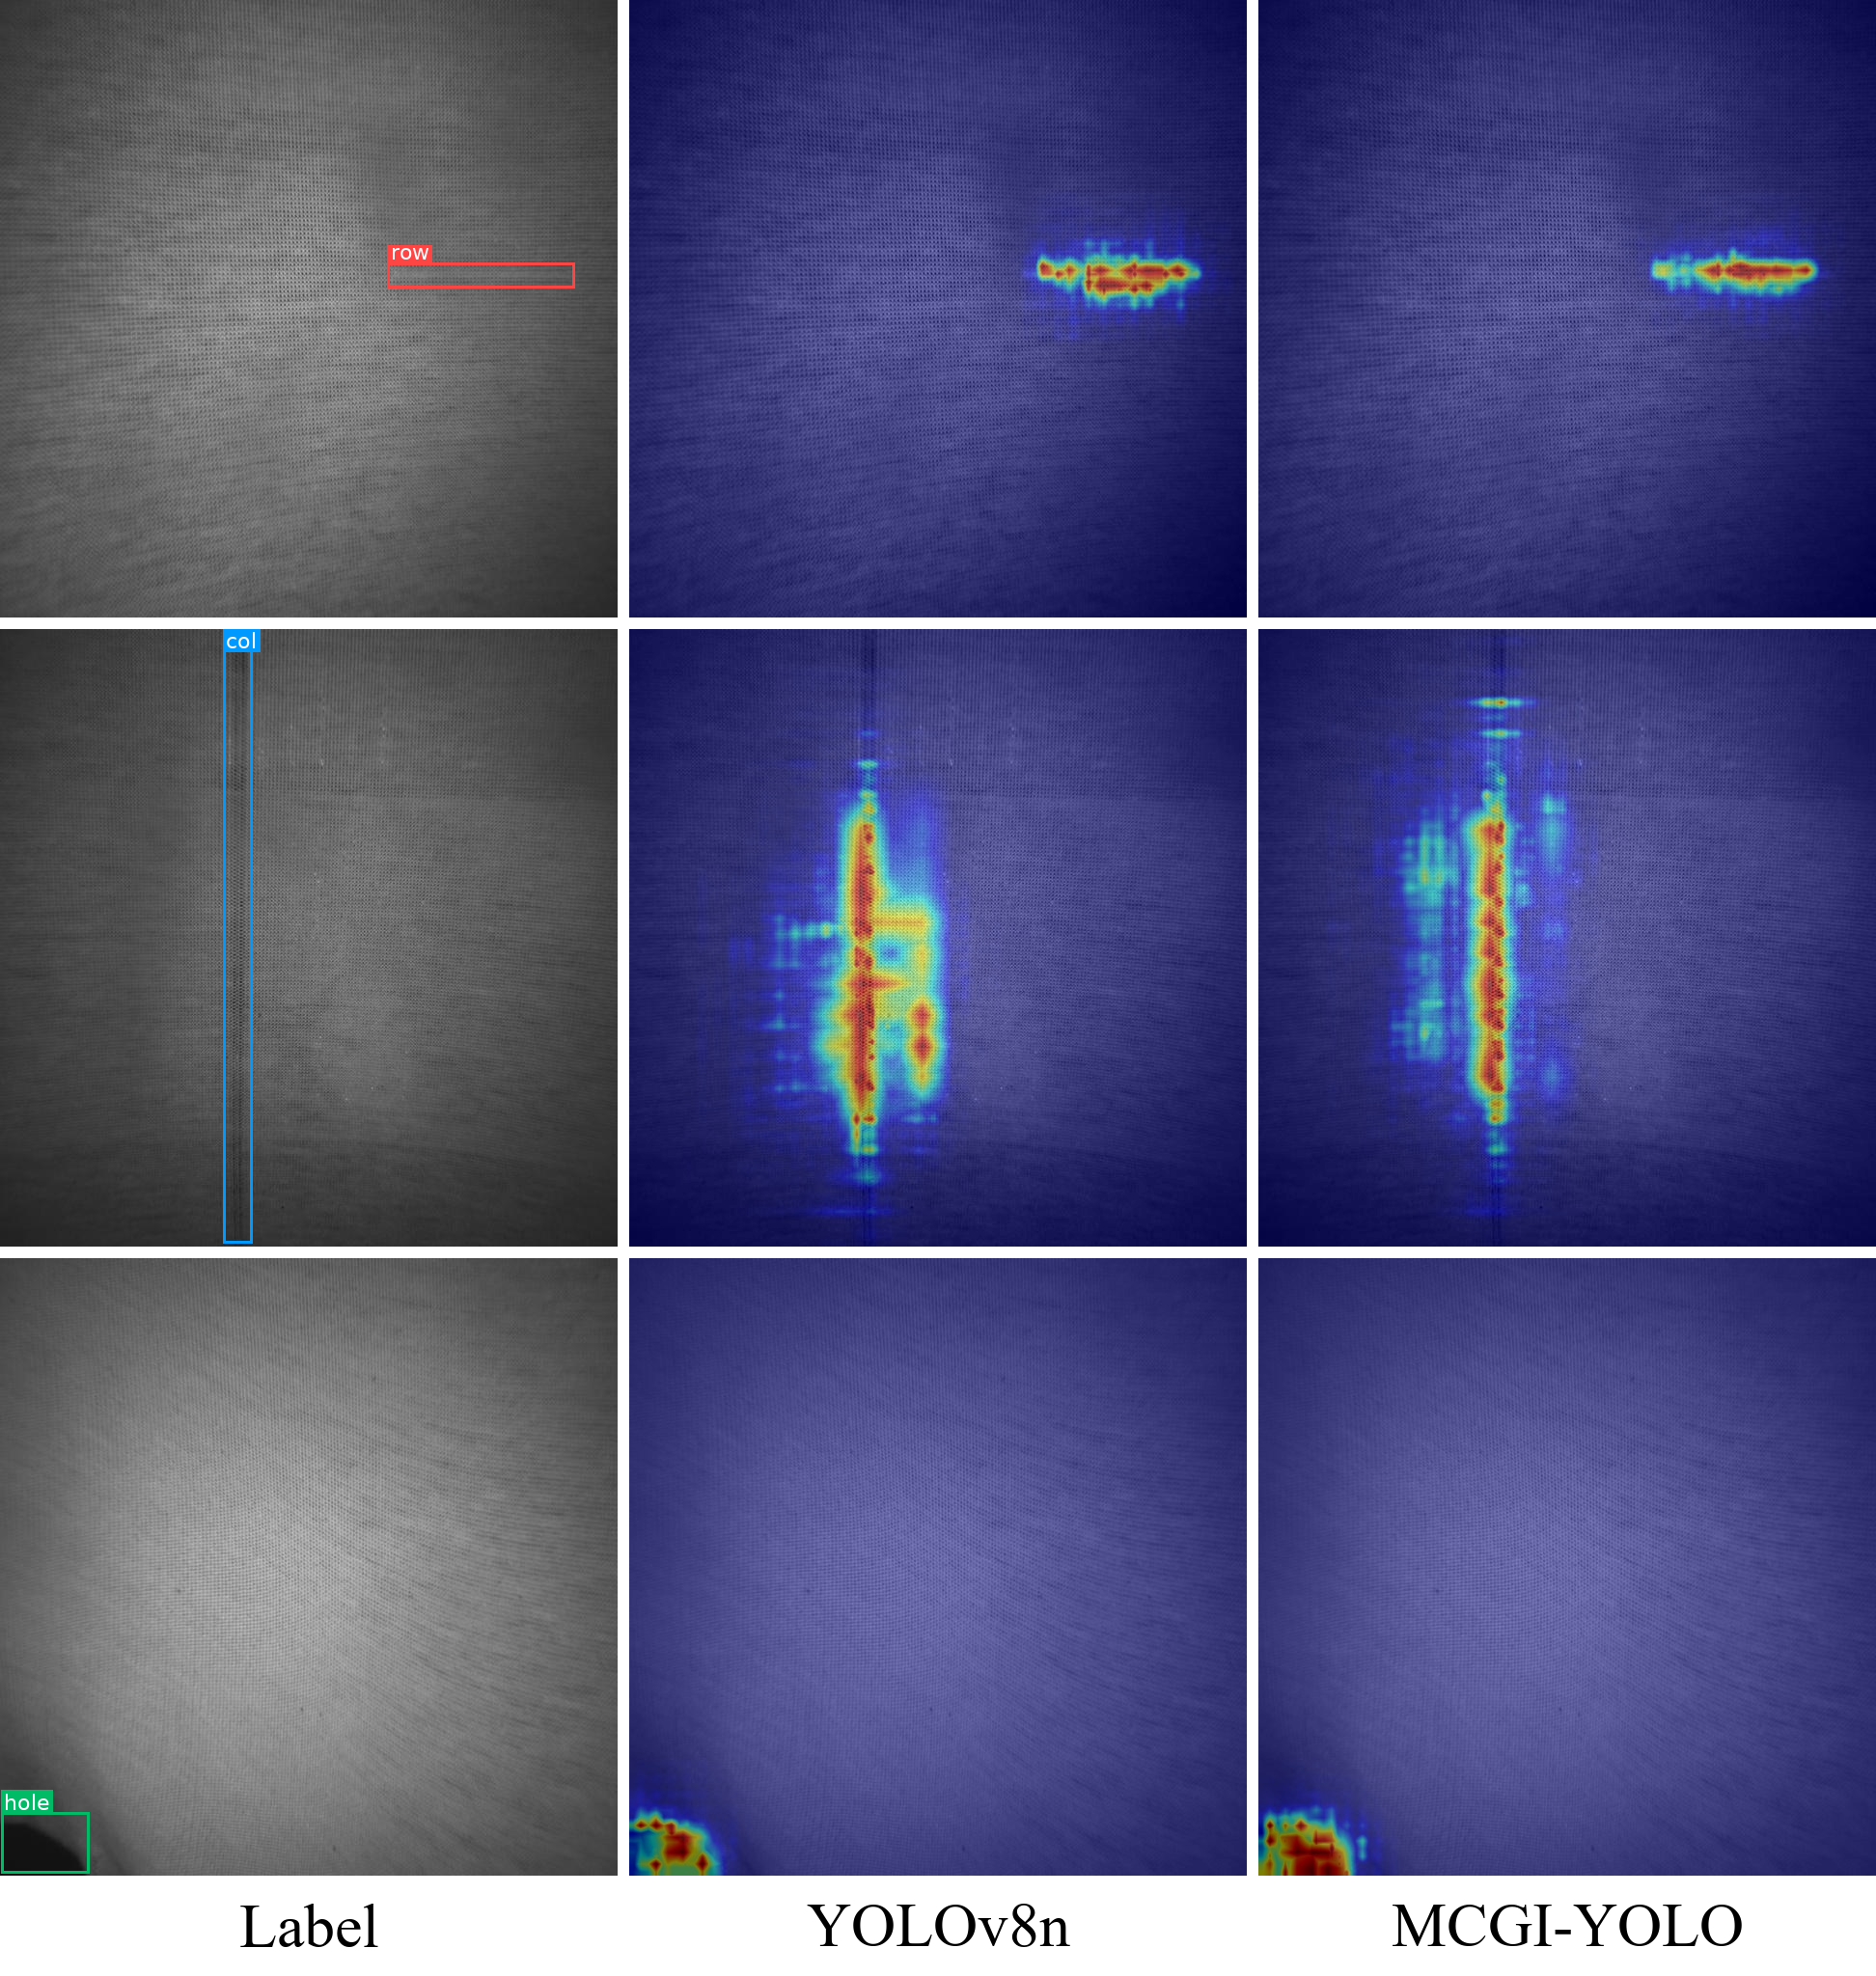
\includegraphics[width=\columnwidth]{fig7.png}
\caption{Feature visualization of YOLOv8n and \model. From left to right: ground-truth annotations (Label), YOLOv8n, and \model.}
\label{fig:heatmaps}
\end{figure}

\FloatBarrier
\bibliographystyle{IEEEtran}
\bibliography{references}

\begin{IEEEbiography}[{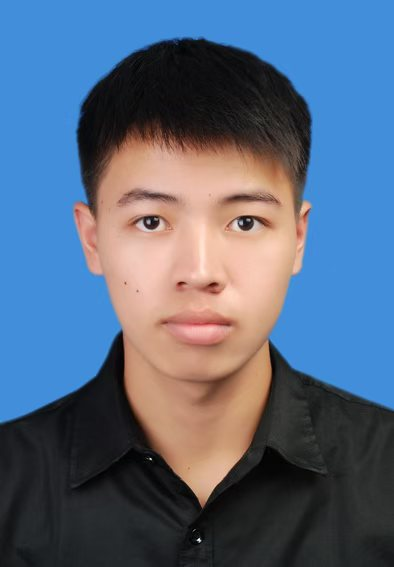
\includegraphics[width=1in,height=1.25in,clip,keepaspectratio]{a1.jpg}}]{Kangzhao Tan}
received the B.S. degree in computer science and technology from Guangzhou University, Guangzhou, China, in 2022. From 2022 to 2024, he worked as a cloud computing R\&D engineer with Sangfor Technologies Inc., Shenzhen, China. He is currently pursuing the M.S. degree in computer technology with the School of Computer Science, Guangdong University of Technology, Guangzhou, China.

His research interests include deep learning, computer vision, and industrial defect detection.
\end{IEEEbiography}

\begin{IEEEbiography}[{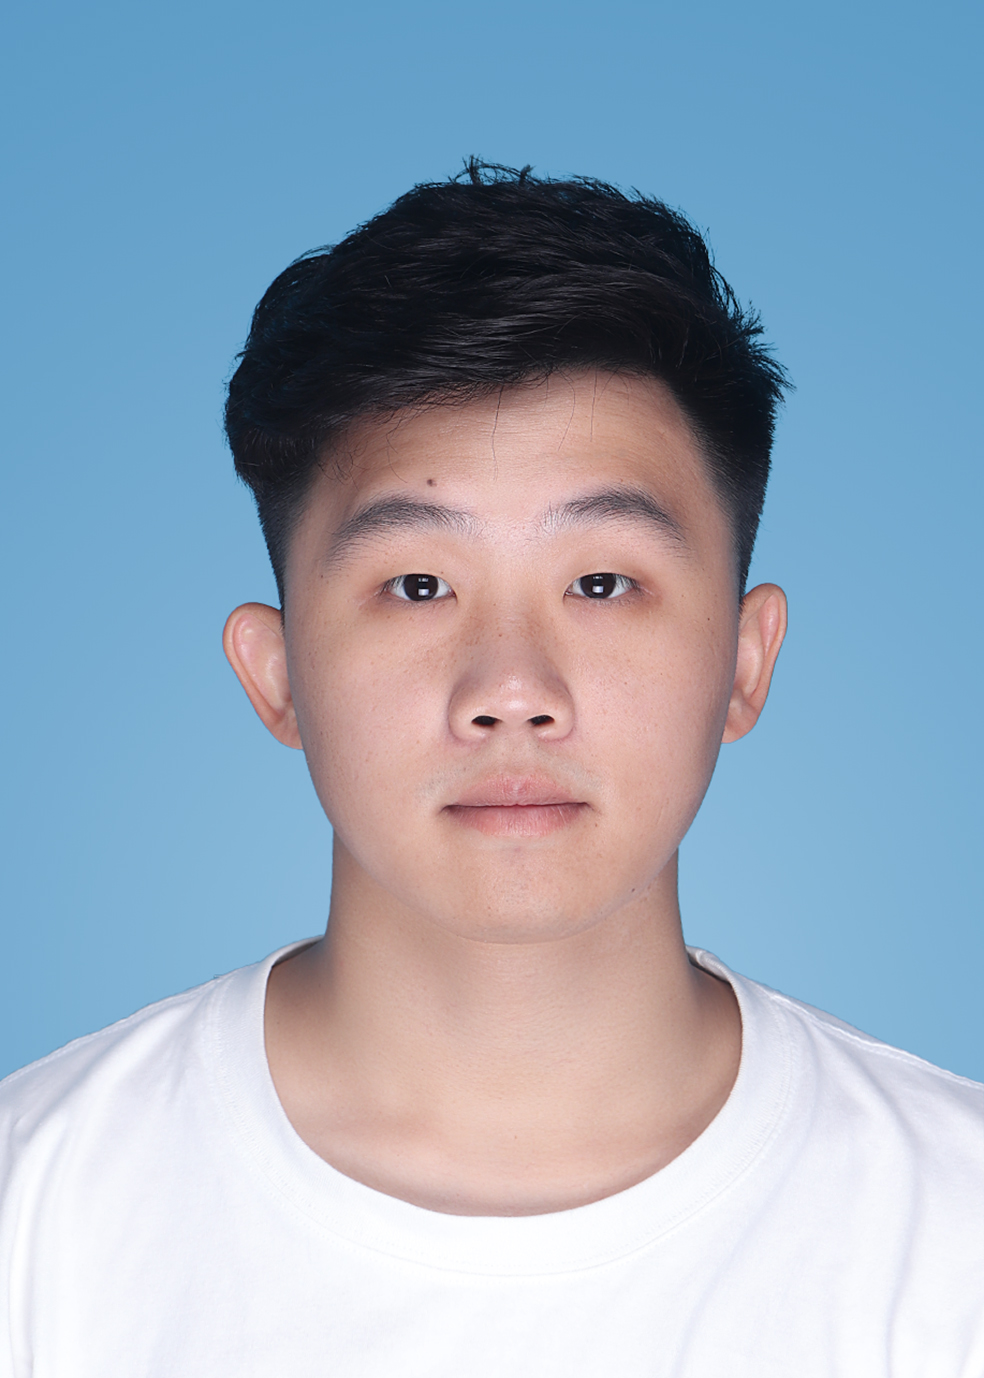
\includegraphics[width=1in,height=1.25in,clip,keepaspectratio]{a2.jpg}}]{Jiarui Zhang}
received the B.S. degree in electrical engineering and automation from Guangdong Polytechnic Normal University, Guangzhou, China, in 2021. He is currently pursuing the M.S. degree in software engineering with the School of Computer Science, Guangdong University of Technology, Guangzhou, China.

His research interests include electronic circuit design and intelligent Internet of Things.
\end{IEEEbiography}

\begin{IEEEbiography}[{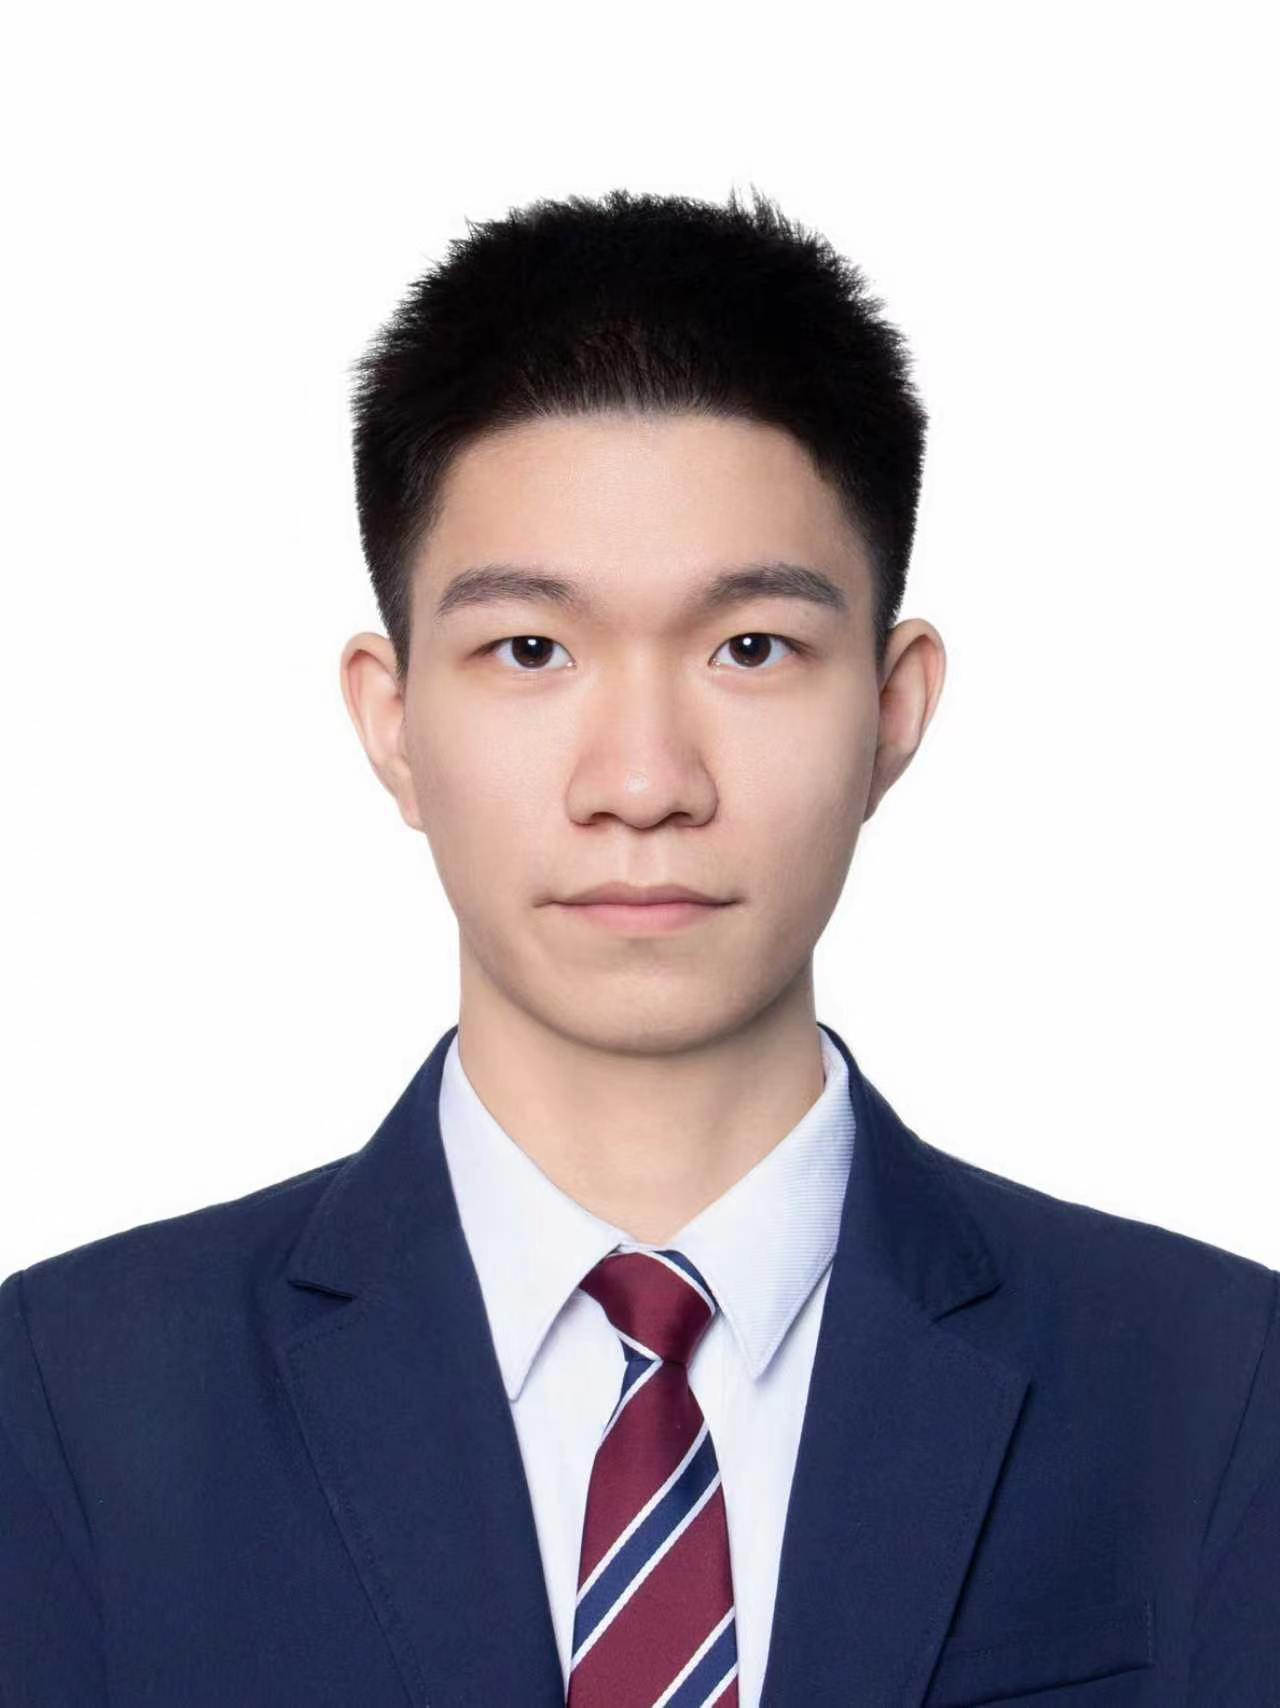
\includegraphics[width=1in,height=1.25in,clip,keepaspectratio]{a3.jpg}}]{Junjie Yu}
received the B.S. degree in computer science and technology from Hunan University of Finance and Economics, Changsha, China, in 2025. He is currently pursuing the M.S. degree in computer technology at Guangdong University of Technology, Guangzhou, China.

His research interests include image processing and edge computing.
\end{IEEEbiography}

\begin{IEEEbiography}[{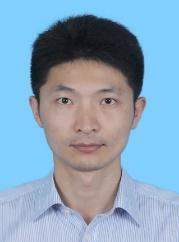
\includegraphics[width=1in,height=1.25in,clip,keepaspectratio]{a4.jpg}}]{Heng Wu}
received the B.S. degree in electronic and information engineering from Wuhan University of Science and Technology, Wuhan, China, in 2009, and the M.S. degree in optics and the Ph.D. degree in mechanical manufacturing and automation from South China University of Technology, Guangzhou, China, in 2012 and 2017, respectively.

He is currently an associate professor with the School of Automation, Guangdong University of Technology. His research interests include optical imaging, optical measurement, machine vision, and image processing.
\end{IEEEbiography}

\begin{IEEEbiography}[{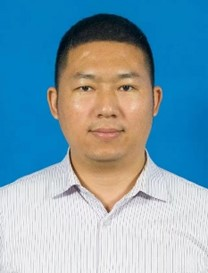
\includegraphics[width=1in,height=1.25in,clip,keepaspectratio]{a5.jpg}}]{Jing Lin}
received the B.S. degree in computer science and technology and the M.S. degree in software engineering from Guangdong University of Technology, Guangzhou, China, in 2003 and 2006, respectively.

Since graduation, he has served as an assistant engineer, engineer, and senior engineer. He is currently a senior engineer with the Classroom Management Center, Guangdong University of Technology. His research interests include information system project management, system informatization, and the intelligent Internet of Things.
\end{IEEEbiography}

\begin{IEEEbiography}[{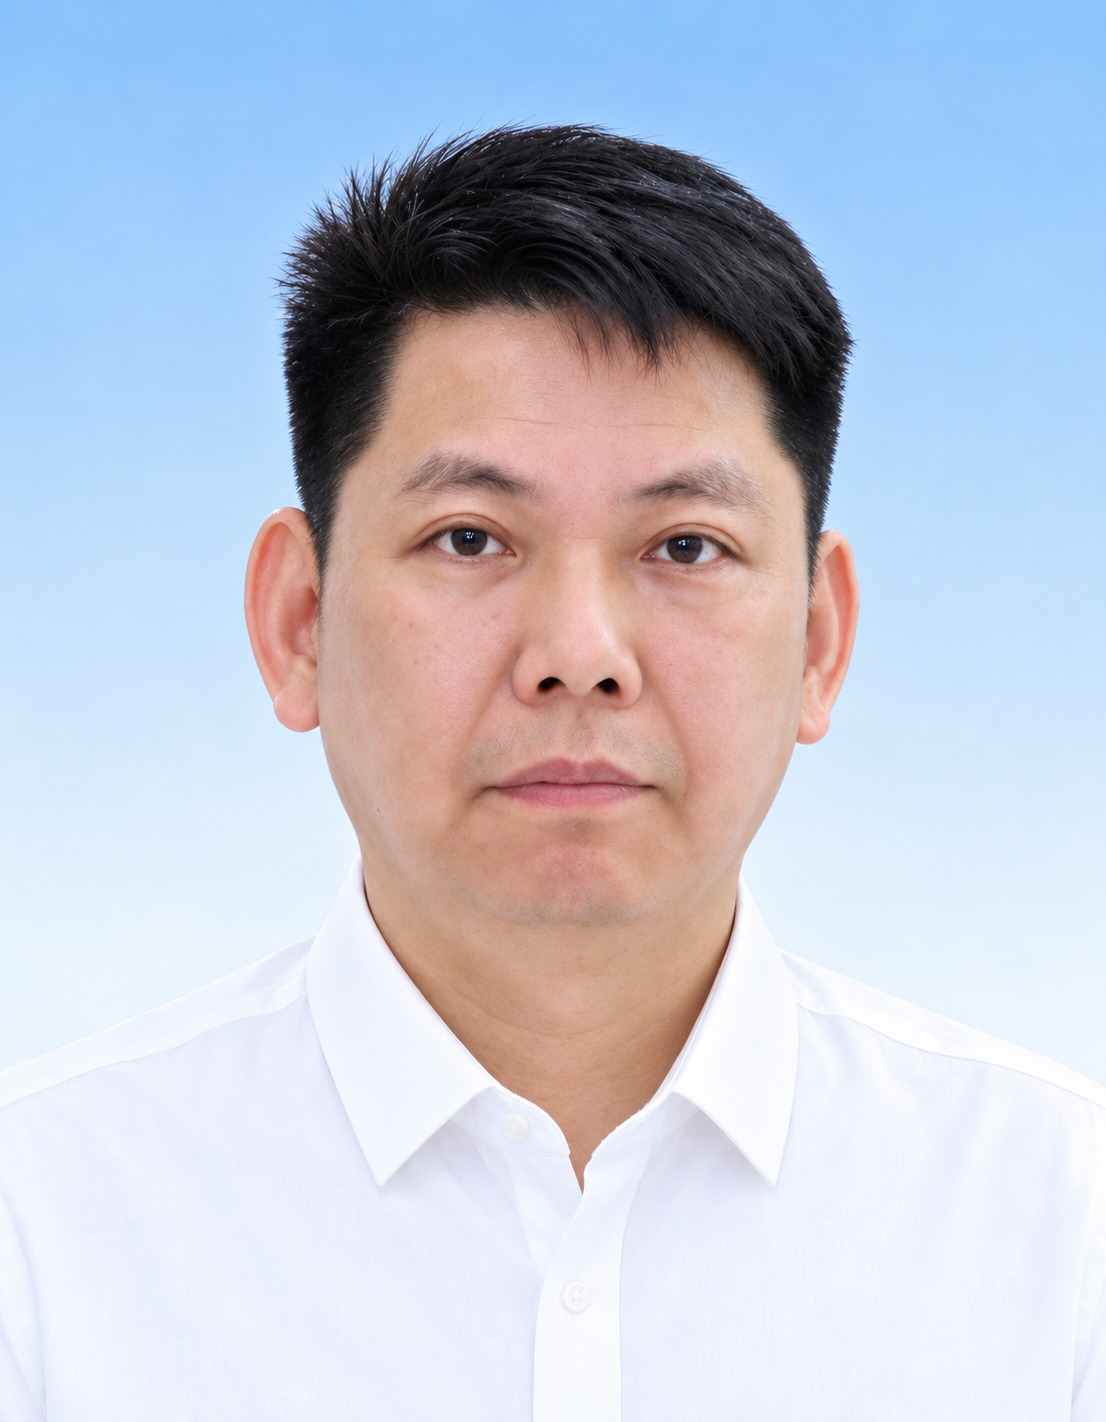
\includegraphics[width=1in,height=1.25in,clip,keepaspectratio]{a6.jpg}}]{Diyu Li}
received the B.S. degree from South China Agricultural University, Guangzhou, China, in 1996, and the M.S. degree in business administration from Lanzhou University, Lanzhou, China, in 2009.

In 2017, he founded Guangzhou Vinsome Automation Technology Co., Ltd., Guangzhou, China. His research interests include artificial intelligence and industrial automation.
\end{IEEEbiography}

\begin{IEEEbiography}[{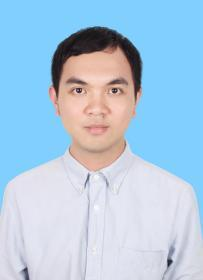
\includegraphics[width=1in,height=1.25in,clip,keepaspectratio]{a7.jpg}}]{Chunhua He}
received the B.S. degree in microelectronics from Sun Yat-sen University, Guangzhou, China, in 2010, and the M.S. and Ph.D. degrees in microelectronics from Peking University, Beijing, China, in 2013 and 2018, respectively.

From 2013 to 2017, he was an engineer with the No. 5 Electronics Research Institute, Ministry of Industry and Information Technology, Guangzhou, China. From 2017 to 2019, he was an engineer with Midea Group, Foshan, China. From 2019 to 2021, he was a senior engineer with Guangzhou 37 Degree Smart Home Co., Ltd., Guangzhou, China. He joined the School of Computer Science, Guangdong University of Technology, Guangzhou, China, in 2021, where he is currently a professor. His research interests include the design and application of MEMS sensors and artificial intelligence algorithms.
\end{IEEEbiography}

\end{document}
